\documentclass[12pt, oneside]{article}
\usepackage{geometry}
\usepackage[utf8]{inputenc}
\usepackage{setspace}
\usepackage{times}
\usepackage{url}
\usepackage{multirow}
\usepackage{fancyhdr}
\usepackage{indentfirst}
\usepackage[german]{babel}
\usepackage{glossaries}
\usepackage{longtable}
\usepackage{graphicx}
\usepackage[natbibapa]{apacite}
\usepackage[font=small,labelfont=bf]{caption}
\usepackage{booktabs}

\geometry{
 a4paper,
 left=30mm,
 top=25mm,
 right=25mm,
 bottom=20mm,
 footskip=15pt,
}

\graphicspath{ {./images/} }

\urlstyle{same}
\setstretch{1.3} % Define Line Spacing


\pagestyle{fancy} % Allow for customizing header and footer
% Customize footer for page number location
\fancyhf{}
\fancyfoot{}
\fancyhead[R]{Yannick Hutter}
\fancyhead[L]{Bachelorthesis}
\fancyfoot[R]{\thepage}
\renewcommand{\headrulewidth}{0pt} % Remove footer line

 \makeglossaries

 \newglossaryentry{dsr}
 {
     name=DSR,
     description={Design science Research}
 }
 
 \newglossaryentry{covid19}
 {
     name=COVID-19,
     description={Coronavirus-Krankheit-2019 ~\citep{covid19}}
 }
 \newglossaryentry{bfs}
 {
     name=BFS,
     description={Bundesamt für Statistik}
 }
 
 \newglossaryentry{foph}
 {
     name=FOPH,
     description={Federal Office of Public Health}
 }
 \newglossaryentry{fhgr}
 {
     name=FHGR,
     description={Fachhochschule Graubünden}
 }
 \newglossaryentry{svi}
 {
     name=SVI,
     description={Social Vulnerability Index}
 }
 \newglossaryentry{who}
 {
     name=WHO,
     description={World Health Organisation}
 }

\begin{document}
\pagenumbering{roman}
\begin{titlepage}
	\begin{center}
		\Huge
		\textbf{Bachelorthesis}\\
		\vspace{0.5cm}
		\LARGE
		Analyse und Implementierung eines personalisierbaren Corona Dashboards für Millenials

		\vspace{1.5cm}
		\normalsize
		\textbf{Yannick Hutter}\\
		\textbf{Digital Business Management Klasse 18tz}\\
		\textbf{Talackerstrasse 8}\\
		\textbf{8887 Mels}\\
		\textbf{yannick.hutter@stud.fhgr.ch}\\


		\vfill
		Referrent: Daniel Klinkhammer\\
		Korefferent: Michael Burch\\

		\vspace{0.8cm}


		Digital Business Management\\
		Fachhochschule Graubünden\\
		Mels, April 2022
	\end{center}
\end{titlepage}

\clearpage
\section*{Abstract}
TODO


\clearpage
\tableofcontents

\clearpage
\listoffigures
\listoftables

\clearpage
\printglossaries

\pagenumbering{arabic}

\clearpage
\section{Einleitung}
In Bezug auf den Schweregrad gab es in der Schweiz seit der Spanischen Grippe im Jahr 1918 keine vergleichbaren Pandemien mehr. Kasbar Staub bezeichnet den Zeitraum von 1918 - 2020, in welchem es keine verheerenden Pandemien für die Schweiz gab, als \textit{Pandemic Gap in Switzerland} (siehe Abbildung \ref{fig:pandemic_gap_switzerland}). Mit dem Auftreten der neusten Pandemie im Jahr 2019, bekannt unter dem Namen \gls{covid19} steht die Schweiz, sowie auch der Rest der Welt vor neuen Herausforderungen.

\begin{figure}[h]
    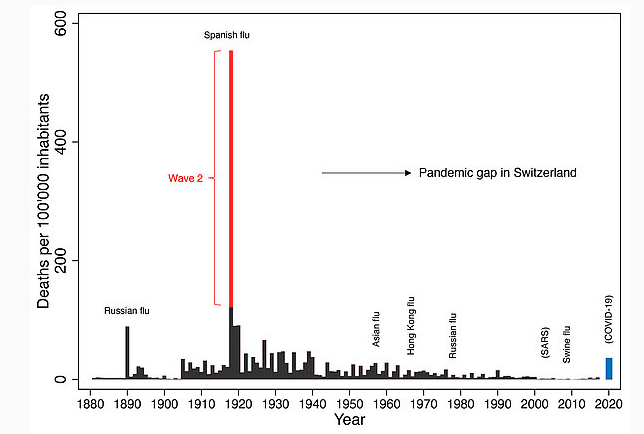
\includegraphics[width=12cm]{images/pandemic_gap_switzerland.png}
    \centering
    \caption{Visualisierung Pandemic Gap in Switzerland ~\citep{switzerland_pandemic_gap}}
    \label{fig:pandemic_gap_switzerland}
\end{figure}


Gemäss der Studie von Statista, welche Epidemien und Pandemien aus dem Jahr 1918 bis 2021 miteinander vergleicht, hebt sich Corona mit rund 5000 krankheitsbedingten Todesfällen pro Tag merklich von anderen Virusvarianten ab (siehe Abbildung \ref{fig:daily_deaths_due_to_contamination}).

\begin{figure}[h]
    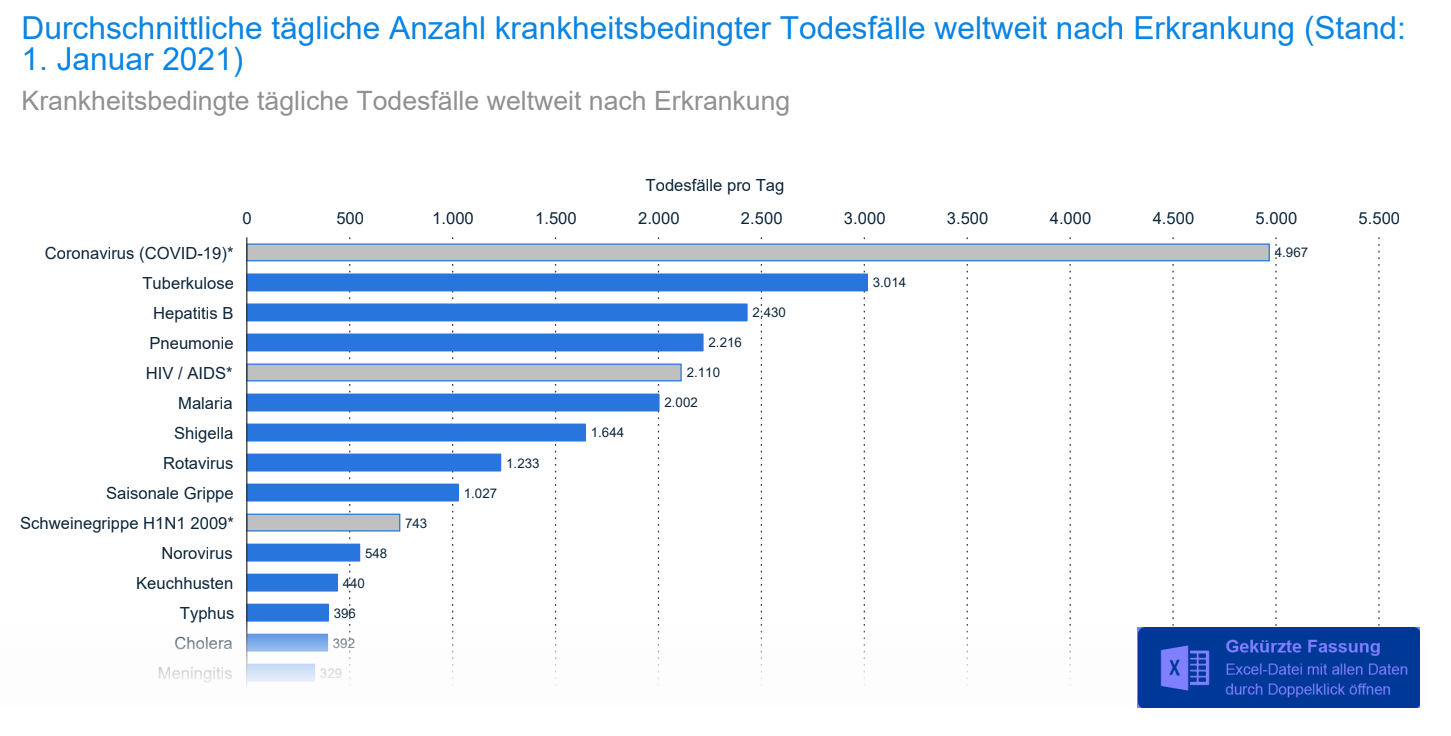
\includegraphics[width=12cm]{images/daily_deaths_after_contamination.png}
    \centering
    \caption{Durchschnittliche tägliche Anzahl krankheitsbedingter Todesfälle weltweit nach Erkrankung (Stand:
1. Januar 2021) ~\citep[S. 6]{worldwide_epidemic_cases_study}}
    \label{fig:daily_deaths_due_to_contamination}
\end{figure}

Ein zentrales Mittel zur Sensibilisierung der allgemeinen Bevölkerung in Bezug auf den Schweregrad der Pandemie sind hierbei \textbf{Datenvisualisierungen} und insbesondere \textbf{Dashboards}. Dies bestätigt ebenfalls Barbazza in seinem Paper, welche die Erfahrungen von 33 nationalen Teams in Bezug auf die Erstellung von Corona spezifische Dashboards im Rahmen einer qualitativen Studie auswertete. Gemäss dem Paper geht hevor, dass Regierungen in der europäischen WHO Region primär ein Dashboard nutzten, um Corona spezifische Daten der Öffentlichkeit mitzuteilen ~\citep[S. 2]{barbazza}. Barbazza identifizierte im Rahmen von qualitativ durchgeführten Experteninterviews mit Personen welche für die Erstellung von Dashboards verantwortlich waren zwei Problematiken. Zum einen wurden die Dashboards für die breite Öffentlichkeit und nicht für eine dedizierte Zielgruppe konzipiert, zum anderen gab es keine effiziente Möglichkeit um an das Feedback der Nutzergruppe zu gelangen ~\citep[S. 14-15]{barbazza}. Die vorliegende Arbeit untersucht diese Problematiken mit der Umsetzung eines Corona Dashboards für die Zielgruppe der Millenials.


\subsection{Stand der Forschung}
 Eine Studie von Statista zum Thema \gls{covid19} zeigt auf, dass die Suchbegriffe ``Corona`` sowie  ``\gls{covid19}`` sehr präsent sowohl bei Medienberichten als auch bei Google-Anfragen sind (siehe Abbildung \ref{fig:covid_term_public_media_presence}).
 
\begin{figure}[h]
    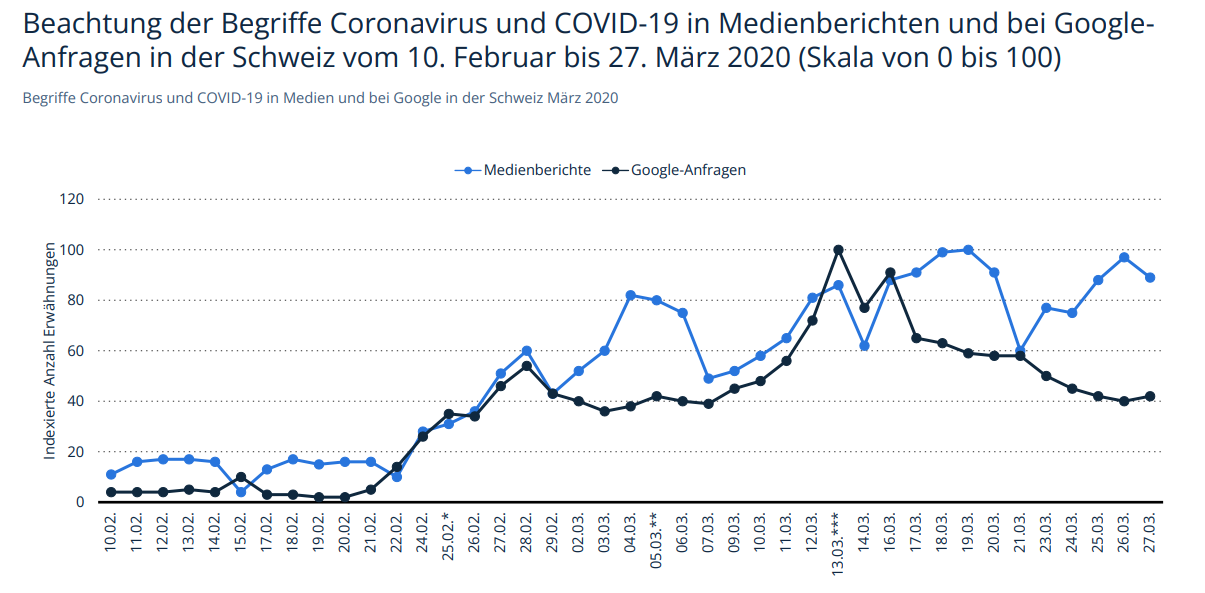
\includegraphics[width=12cm]{images/covid_term_public_media_presence.png}
    \centering
    \caption{Beachtung der Corona Begrifflichkeiten in Medienberichten und bei Google-Anfragen vom 10. Februar 2020 bis 27. März 2020 ~\citep[S. 50]{covid_term_public_media_presence}}
    \label{fig:covid_term_public_media_presence}
\end{figure}
 
Nachfolgend wird auf die wichtigsten bereits bestehenden Studien eingegangen, welche sich mit  \textbf{Datenvisualisierungen} sowie \textbf{Dashboards} im Zusammenhang mit Corona beschäftigen.
 
 \subsubsection{Die Landschaft der Corona Datenvisualisierungen} \label{ch:landscape_of_covid_data_visualization}
 Eine massgebende Studie um einen Überblick über die Landschaft der Corona Datenvisualisierungen zu erhalten, ist die Studie von Zhang. Bei dieser Studie wurden rund 668 Corona Datenvisualisierungen im Zeitraum vom 22. Januar bis zum 31. Juli 2020 analysiert. Ein wichtiges Auswahlkriterium bei diesen Visualisierungen war, dass die allgemeine Bevölkerung als Zielgruppe im Fokus stand. Anschliessend wurden diese Visualisierungen sowohl mittels \textit{deduktiver} als auch \textit{induktiver} Codierung in Form eines Codebooks zusammengefasst ~\citep[S. 3]{yixuan_zhang}. Nebst dem Codebook erstellte Zhang zudem ein Rahmenwerk zum Verständnis von Datenvisualisierungen in Krisenzeiten (siehe Abbildung \ref{fig:zhang_conceptual_framework}).
 
 
 \begin{figure}[h]
    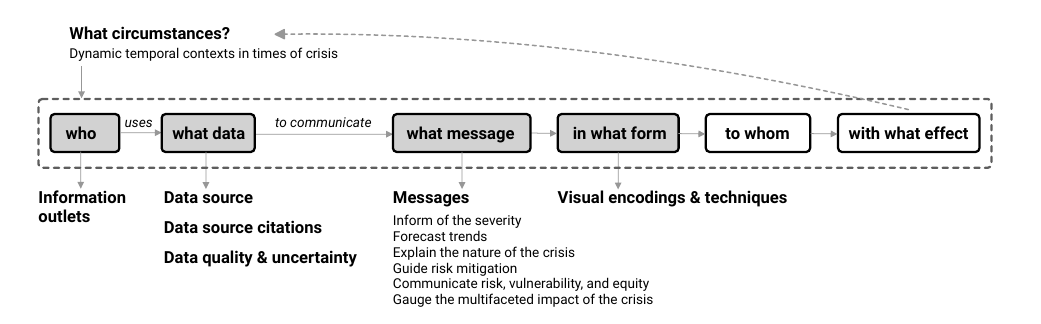
\includegraphics[width=12cm]{images/zhang_conceptual_framework.png}
    \centering
    \caption{Konzeptionelles Framework zum Verständnis von Datenvisualisierungen in Krisenzeiten ~\citep[S. 4]{yixuan_zhang}}
    \label{fig:zhang_conceptual_framework}
\end{figure}
 
 
 Die Studie von Zhang fokussierte sich hierbei primär auf die ersten vier Aspekte des Modells (who uses what data to communicate what message in what form). Im erstellten Codebook finden sich diese vier Aspekte ebenfalls wieder. Hierbei kann der Aspekt \textbf{who} mithilfe der Metainformationen ``Publisher`` sowie ``URL`` beantwortet werden (siehe Abbildung \ref{fig:zhang_codebook_metadata}).
 
 \begin{figure}[h]
    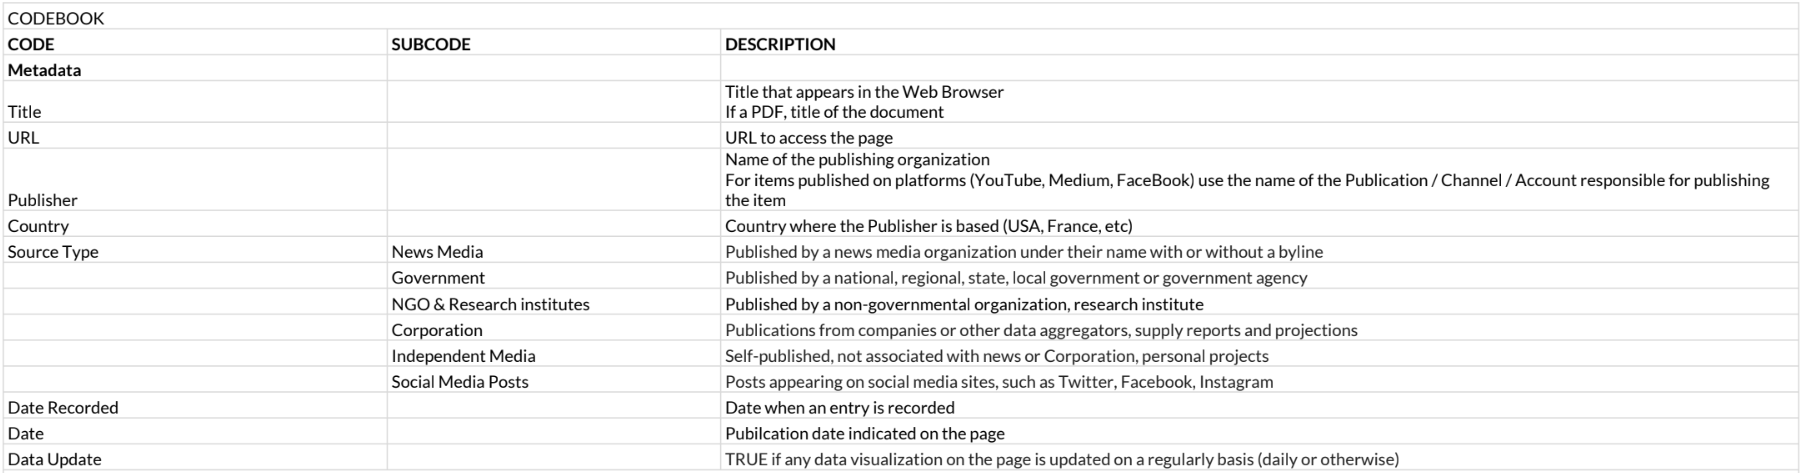
\includegraphics[width=12cm]{images/zhang_codebook_metadata.png}
    \centering
    \caption{Ausschnitt Metadaten aus dem Codebook von Zhang ~\citep{zhang_codebook}}
    \label{fig:zhang_codebook_metadata}
\end{figure}

Der Aspekt \textbf{what data} ist durch die Sektion ``Data Handling`` abgedeckt, welcher Informationen bezüglich der Datenquelle etc. aufweist (siehe Abbildung \ref{fig:zhang_codebook_data_handling}).

\begin{figure}[h]
    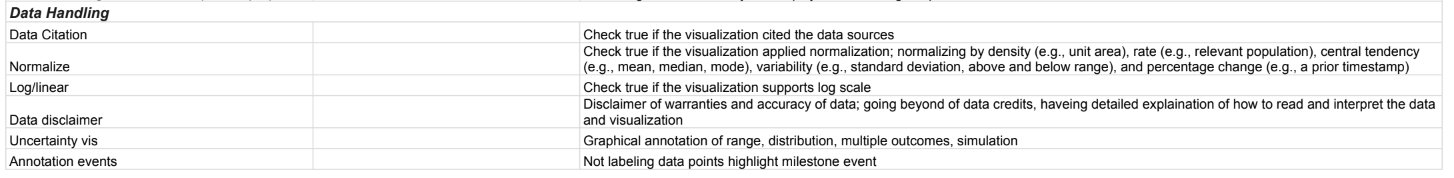
\includegraphics[width=12cm]{images/zhang_codebook_data_handling.png}
    \centering
    \caption{Ausschnitt Data Handling aus dem Codebook von Zhang ~\citep{zhang_codebook}}
    \label{fig:zhang_codebook_data_handling}
\end{figure}

 \textbf{What messages} sind durch die ``Intended Message`` Kategorie, welche mithilfe deduktiver sowie induktiver Codierung entstand, abgedeckt (siehe Abbildung \ref{fig:zhang_codebook_intended_message}).

\begin{figure}[h]
    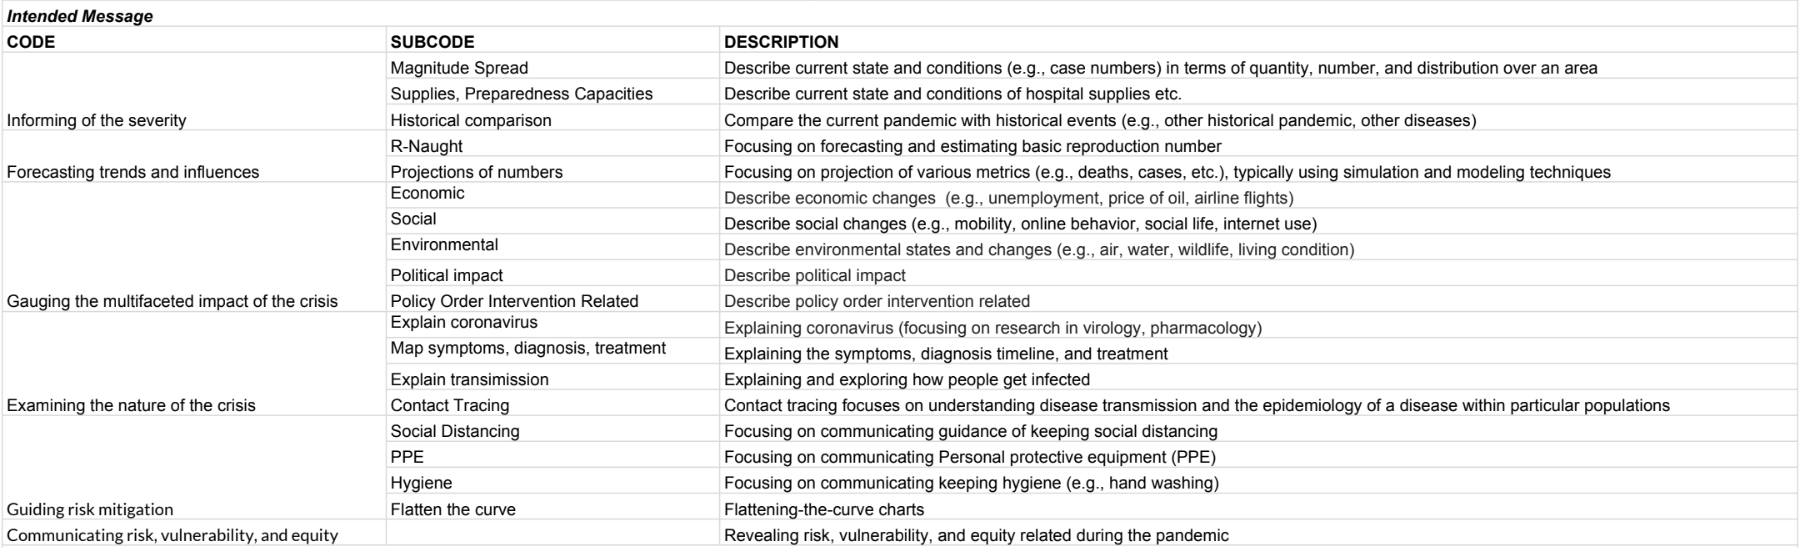
\includegraphics[width=12cm]{images/zhang_codebook_intended_message.png}
    \centering
    \caption{Ausschnitt Intended Message aus dem Codebook von Zhang ~\citep{zhang_codebook}}
    \label{fig:zhang_codebook_intended_message}
\end{figure}

 Der letzte Aspekt \textbf{in what form} kann ebenfalls aus dem Codebook entnommen werden. Zhang hat hierbei unter der Kategorie ``Type of Visualization`` verschiedene Visualisierungsarten wie zum Beispiel Liniendiagramme etc. aufgeführt (siehe Abbildung \ref{fig:zhang_codebook_type_of_visualization}).
 
 
\begin{figure}[h]
    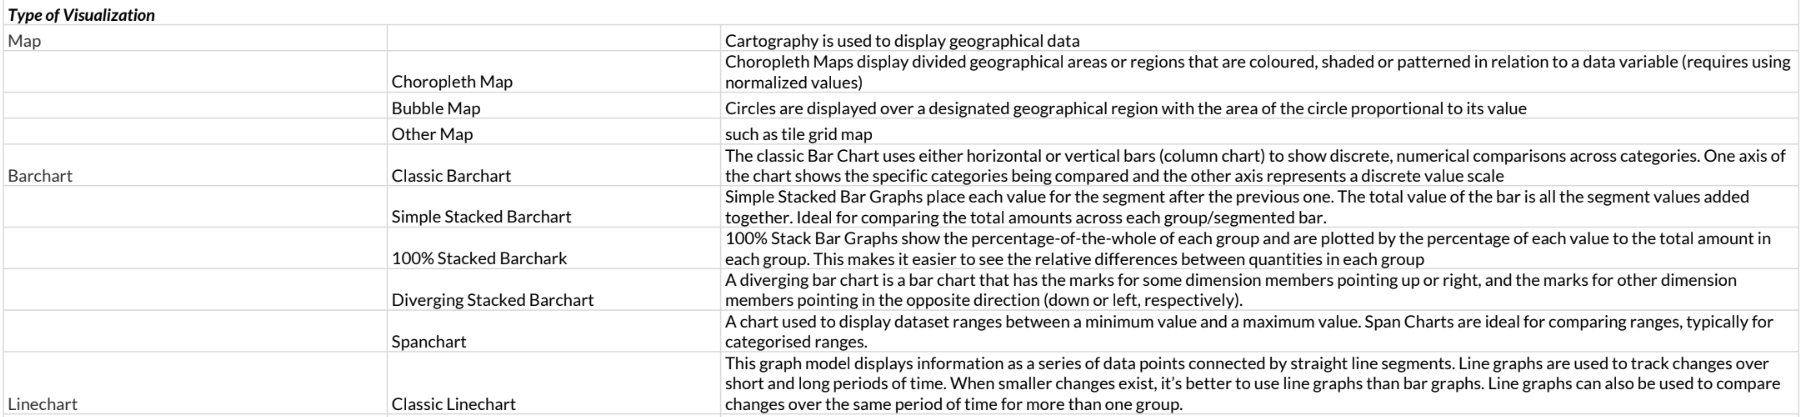
\includegraphics[width=12cm]{images/zhang_codebook_type_of_visualization.png}
    \centering
    \caption{Ausschnitt Type of Visualization aus dem Codebook von Zhang ~\citep{zhang_codebook}}
    \label{fig:zhang_codebook_type_of_visualization}
\end{figure}

Das Codebook bietet somit eine solide Grundlage um die Landschaft der Corona Datenvisualisierungen zu erfassen. Zudem kann es aufgrund seiner strukturierten Kategorien für weiterführende \textbf{Datenauswertungszwecke} verwendet werden.   
 
 
\subsubsection{Corona-Dashboards} \label{ch:introduction_corona_dashboards}
Barbazza führte in Bezug auf Corona Dashboards eine qualitative Studie durch, welche die Erfahrungen und Eindrücke von 33 nationalen Teams in Bezug auf die Konzeption und Umsetzung von Corona Dashboards untersuchte. Barbazza untersuchte hierbei zwei zentrale Hauptaspekte (siehe Abbildung \ref{fig:barbazza_method_design}). 


\begin{figure}[h]
    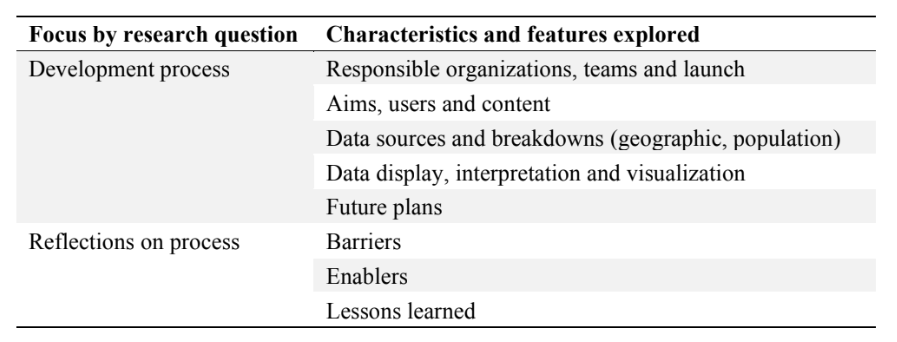
\includegraphics[width=12cm]{images/barbazza_method_design.png}
    \centering
    \caption{Hauptfokuspunkte der Studie von Barbazza ~\citep[S. 4]{barbazza}}
    \label{fig:barbazza_method_design}
\end{figure}

Zum einen wurde der Entwicklungsprozess eines Corona Dashboards analysiert. Nachfolgend wurden Barrieren (Dinge welche den Entwicklungsprozess behinderten), Enablers (Dinge welche den Entwicklungsprozess vorangetrieben haben) sowie Lessons learned identifiziert. Die Studie von Barbazza bietet somit eine gute Grundlage um das bestehende Feedback in Bezug auf Corona Dashboard Design einzuholen.

Anders als Barbazza fokussierte sich Ivankovi{\'c} hingegen explizit auf \textit{webbasierte} Dashboards. Konkret wurden hierbei Aspekte wie Funktion (Purpose), Inhalt und Daten (What) sowie die eigentliche Visualisierung (how they communicate COVID-19 data) untersucht. Aus den insgesamt 158 untersuchten Dashboards wurden anschliessend die Gemeinsamkeiten evaluiert. Hieraus entstanden 7 zentrale Merkmale von interaktiven webbasierten Dashboards (siehe Abbildung \ref{fig:ivankovic_characteristics_of_webbased_dashboards}). Diese Merkmale bildeten anschliessend die Grundlage, um die 158 untersuchten Dashboards zu bewerten ~\citep{ivankovic}. Ivankovi{\'c} bietet somit ein Bewertungsraster in Bezug auf interaktive, webbasierte Corona Dashboards an.


 \begin{figure}[h]
    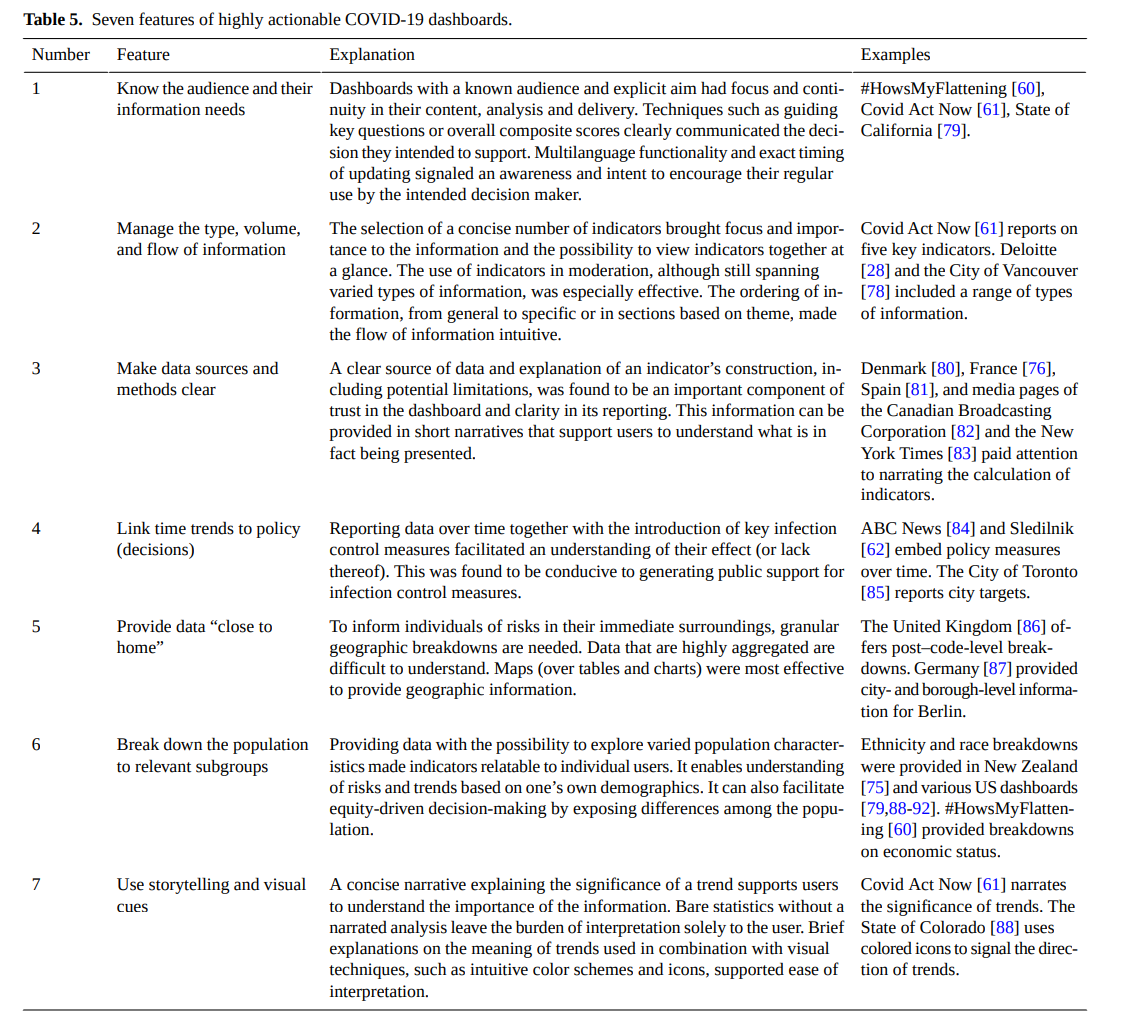
\includegraphics[width=10cm]{images/ivankovic_dashboard_characteristics.png}
    \centering
    \caption{Merkmale von interaktiven, webbasierten Dashboards gemäss Ivankovi{\'c} ~\citep[S. 12]{ivankovic}}
    \label{fig:ivankovic_characteristics_of_webbased_dashboards}
\end{figure}


\subsection{Themenabgrenzung und Zielsetzung}
Der Bereich der Datenvisualisierungen im Zusammenhang mit \gls{covid19} ist umfassend. Dashboards erlauben eine verdichtete Sicht auf die relevantesten Informationen, welche mit Hilfe von Datenvisualisierungen bereit gestellt werden können. Ein Problem welches Barbazza bereits in Ihrer Studie entdeckte, war dass die meisten Dashboards für eine allgemeine Zielgruppe ausgerichtet sind. Die vorliegende Arbeit hat daher zum Ziel, ein personalisierbares Dashboard für die Zielgruppe der Millenials zu entwickeln.

\subsection{Forschungsfrage}
Die vorliegende Arbeit möchte die Erstellung eines personalisierbaren Corona Dashboards für die Zielgruppe Millenials erforschen. Daher wurde folgende übergeordnete Fragestellung formuliert:

\begin{center}
\textbf{Wie stellen sich Millennials ein personalisierbares Corona Dashboard vor?}
\end{center}

Um diese Forschungsfrage abzudecken, wurden folgende untergeordnete Fragestellungen formuliert:

\begin{center}
\textbf{Welche Visualisierungsarten in Bezug auf Corona werden von Millennials gefordert?\\
(untergeordnete Forschungsfrage 1)}
\end{center}

\begin{center}
\textbf{Welche Informationen in Bezug auf Corona werden von Millennials gefordert?\\
(untergeordnete Forschungsfrage 2)}
\end{center}

\begin{center}
\textbf{Welche Personalisierungsmöglichkeiten werden von Millennials in Bezug auf Corona Dashboards gefordert?\\
(untergeordnete Forschungsfrage 3)}
\end{center}

\clearpage
\subsection{Methodische Vorgehensweise}
Da das Ziel der vorliegenden Arbeit die Erstellung eines personalisierbaren Corona Dashboards für Millenials ist, wurde als methodische Vorgehensweise das \gls{dsr} Modell nach Peffers gewählt, welches die Erstellung eines Artefakts zulässt (siehe Abbildung \ref{fig:peffers_dsr_model}).

\begin{figure}[h]
	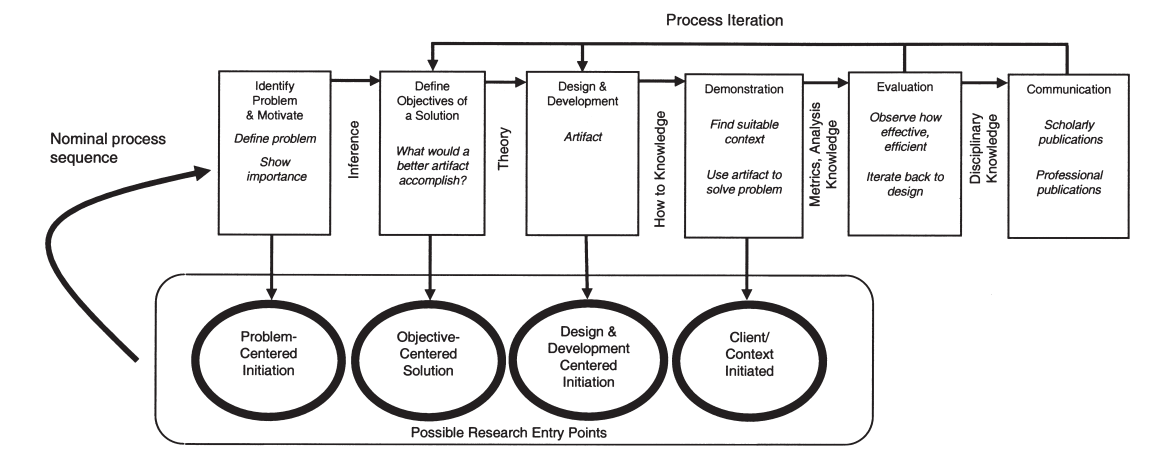
\includegraphics[width=14cm]{images/peffers_dsr_model.png}
	\centering
	\caption{DSR Modell nach Peffers ~\citep[S. 54]{peffers}}
	\label{fig:peffers_dsr_model}
\end{figure}

Das Modell bietet hierbei mehrere Einstiegsmöglichkeiten (siehe ``Possible Research Entry Points``). Der Einstiegspunkt für die vorliegende Arbeit bildet der Punkt \textbf{Design \& Development Centered Initiation}. Dies setzt zugleich auch den Zielfokus der Arbeit auf den Bereich Design und Entwicklung. Um diesen Kernbereich jedoch ausreichend erforschen zu können, werden im Verlaufe der Arbeit die ersten fünf Aktivitäten ``Identify Problem \& Motivation``, ``Define Objective \& Solution``, ``Design \& Development``, ``Demonstration`` sowie ``Evaluation`` behandelt.

\subsubsection{Problem Identification \& Motivation}
In der Aktivität ``Problem Identification \& Motivation`` wird das spezifische Problem, welches gelöst werden soll beschrieben sowie der Nutzen einer möglichen Lösung aufgezeigt ~\citep[S. 52]{peffers}. Als Grundlage für die Problemidentifiaktion dient hierbei die Studie von Barbazza, die Arbeit fokussiert sich hierbei auf die Barrieren in den Bereichen ``Nutzer`` sowie ``Software``. Hauptfokus ist die Erarbeitung eines Dashboards für die Zielgruppe Millenials.

\subsubsection{Define Objective \& Solution}
Bei dieser Aktivität geht es um die Definierung der Ziele ~\citep[S. 52]{peffers}. Hierbei werden in einem ersten Schritt die Anforderungen der Zielgruppe mithilfe eines qualitativen Ansatzes erhoben. Konkret wird hierbei herausgefunden welche Visualisierungsarten und Informationen in Bezug auf Corona von Millenials gefordert werden (untergeordnete Forschungsfrage 1 und 2). Dies wird mithilfe einer Online Umfrage abgedeckt. In einem weiteren Schritt werden die Personalisierungsmöglichkeiten durch ein Nutzerinterview evaluiert (untergeordnete Forschungsfrage 3). Schlussendliche werden sowohl die Online Umfrage, als auch die Nutzerinterviews ausgewertet. Hieraus werden dann die Ziele definiert.

\subsubsection{Design \& Development}
Die Design und Entwicklungsaktivität bildet den Hauptfokus der Arbeit. Aufgrund der definierten Ziele wird ein Corona Dashboard spezifisch für die Zielgruppe der Millenials umgesetzt. Die Umsetzung erfolgt hierbei als Web Applikation und beinhaltet nebst der eigentlichen Visualisierung auch die Datenaufbereitung sowie die Implementierung einer Schnittstelle, womit diese Daten einfach abgerufen werden können.

\subsubsection{Demonstration}
Die Zielgruppe wird im Rahmen dieser Aktivität dazu aufgefordert, diverse Aufgaben mithilfe der Web Applikation zu lösen. Hieraus wird ersichtlich, ob die Web Applikation verständlich und benutzungsfreundlich ist.

\subsubsection{Evaluation}
Die Ergebnisse des aufgabenbezogenen User Testings werden ausgewertet und evaluiert. Grundsätzlich ist gemäss Peffers aufgrund der Ergebnisse ein Rücksprung zur Aktivität ``Define Objective \& Solution`` möglich ~\citep[S. 56]{peffers}, im Rahmen dieser Arbeit wird jedoch auf diesen iterativen Schritt verzichtet.

\clearpage
\section{Webbasierte Corona Dashboards}

\subsection{Dashboard – Ein Begriff mit Ursprung in der Automobilindustrie}
Im Kontext dieser Arbeit wird unter dem Begriff Dashboard die Definition von Duden verwendet. Duden definiert ein Dashboard als: \textbf{Ein Computerprogramm das relevante Informationen zusammenfasst und übersichtlich darstellt} ~\citep{term_definition_dashboard}.


\subsection{Aufbau und Komponenten von webbasierten Dashboards}
Webbasierte Dashboards sind Dashboards, welche über das Internet zugänglich gemacht werden und mit Hilfe eines Webbrowsers dargestellt werden können. Wie herkömmliche Webseiten funktionieren auch webbasierte Dashboards nach dem \textit{Client-Server-Modell} (siehe Abbildung 6). Hierbei sendet der Browser (PC, Smartphone etc.) beim Besuch einer Internet Seite (\url{https://www.covid19.admin.ch/en/overview}) eine Anfrage an den Web Server. Dieser wiederum Antwortet mit dem gewünschten Inhalt (Corona Dashboard). Jedoch benötigt es noch eine dritte, sehr zentrale Komponente, die Datenquelle. In der heutigen Zeit sind Internet Seiten keine starren Textkonstrukte mehr, sie passen sich dynamisch an die Anforderungen des Nutzers an. Besonders für webbasierte Corona Dashboards sind dynamische Daten von enormer Bedeutung. 

Grundsätzlich wird für webbasierte Dashboards mindestens folgende Komponenten benötigt:
\begin{itemize}
    \item Web Server auf welchem die eigentliche Web Applikation läuft und welcher Anfragen entgegennimmt
    \item Datenbank auf welcher die Daten vorhanden sind
    \item Schnittstelle zwischen Datenbank und Webserver, welche die Kommunikation dieser beiden Komponenten ermöglicht
\end{itemize}

\subsection{Vorteile}

Ein grosser Vorteil von webbasierten Dashboards besteht in der grossen Erreichbarkeit der Nutzer. In der heutigen Zeit besitzen die meisten Personen nebst einem Computer ebenfalls über ein Smartphone mit integriertem Browser. Somit ist der Zugriff auf ein webbasiertes Dashboard nebst dem Computer auch über das Smartphone, über ein Tablet etc. möglich. Dies ist von enormer Bedeutung, da man so ortsunabhängig immer auf dem aktuellen Stand ist. Auch können moderne Web Applikationen Gebrauch vom GPS System des Smartphones machen und so standortbezogene Daten liefern. Die Voraussetzung hierzu ist lediglich die Nutzung eines modernen Browsers.

\begin{figure}[ht]
	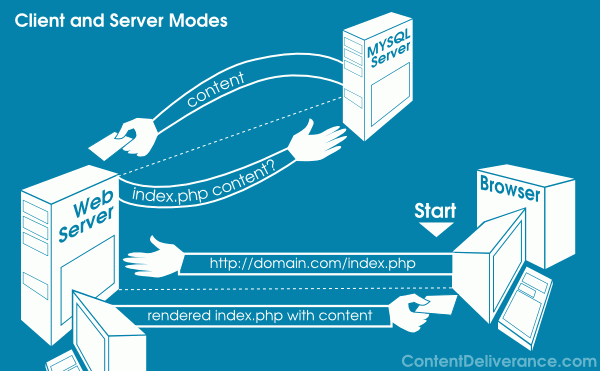
\includegraphics[width=12cm]{images/client_server_model.png}
	\centering
	\caption{Client-Server-Modell ~\citep{client_server_model}}
\end{figure}

\clearpage
\section{Problemidentifizierung und Motivation}
Gemäss Peffers soll der Schritt \textit{Problem Identification \& Motivation} dabei helfen, den Nutzen einer möglichen Lösung aufzuzeigen. Dies wiederum steigert zum einen die Motivation an der Arbeit selbst und sorgt zum anderen dafür, dass die Beweggründe für alle beteiligten Personen verständlich sind ~\citep[S. 52 + 55]{peffers}.


\subsection{Problemidentifikation}
Als Grundlage für die Problemidentifikation dient die Studie von Barbazza. Barbazza hat diverse Probleme in den Bereichen ``Users`` sowie ``Software`` identifiziert. Die wichtigsten Probleme waren hierbei die Entwicklung eines Dashboards für eine breite Zielgruppe, unzureichende Möglichkeiten um an Nutzerfeedback zu kommen sowie die Limitationen der eingesetzten Software in Bezug auf die Auswahl der Datenvisualisierungen und die Anpassungsmöglichkeiten ~\citep[S. 14-15]{barbazza}.

\subsection{Motivation – Erstellung eines personalisierbaren Corona Dashboards für Millennials}
Das Ziel dieser Arbeit ist die Konzeption und Erstellung eines Corona Dashboards für die Zielgruppe Millennials. Hierbei soll konkret ermittelt werden, welche Informationen sowie Visualisierungsarten für die Zielgruppe von Relevanz sind. Zudem soll ein besonderer Aspekt auf die Anpassbarkeit (Personalisierbarkeit) des Corona Dashboards gelegt werden. Die Lösung soll dazu dienen, den Erstellungsprozess von Dashboards in die Hände der Zielgruppe selbst zu legen. Nutzer können hierbei aus einem Katalog von Visualisierungen auswählen und ihr ganz persönliches Dashboard gestalten. Das erstellte Dashboard kann anschliessend an die relevanten Behörden (BAG) gesendet werden und soll so neue Ideen für Dashboard Designs antreiben sowie das Einholen von Feedback fördern.


\clearpage
\section{Identifikation der Anforderungen}
Gemäss Peffers können die Anforderungen sowohl mithilfe einer \textit{qualitativen} als auch \textit{quantitativen} Methodik erhoben werden ~\citep[S. 55]{peffers}. Da die Entwicklung des Artefakts auf eine bestimmte Zielgruppe abzielt und sich mithilfe von qualtativen Methodiken tieferführende Informationen erheben lassen, wurde zur Identifikation der Anforderungen ein \textbf{qualitatives Vorgehen} gewählt. Um die Anforderungen in Bezug auf die definierten Forschungsfragen (siehe Kapitel \ref{ch:introduction_research_question}) zu beantworten, wird zuerst ein geeignetes Untersuchungsinstrument erstellt. Mithilfe des Untersuchungsinstrumentes können anschliessend die Anforderungen ermittelt und ausgewertet werden.

\subsection{Erstellung des Untersuchungsinstrumentes}
Als Basis für die Erstellung des Untersuchungsinstrumentes wurde das Codebook von Zhang verwendet. Das Codebook unterteilt dabei Corona Datenvisualisierungen in verschiedene Kategorien von Nachrichtentypen (siehe Kapitel \ref{ch:introduction_landscape_of_covid_datavisualizations}). Nebst den Nachrichtenkategorien stehen ebenfalls die verwendeten Visualisierungsarten (Liniendiagram, Balkendiagram etc.) zur Verfügung. In einem ersten Schritt wurde das Codebook welches als \gls{csv} Datei zur Verfügung steht ausgewertet.

\subsubsection{Auswertung des Codebooks mithilfe von Jupyter Notebook} \label{ch:analysis_of_codebook}
Für die Auswertung des Codebooks wurde ein Python Jupyter Notebook\footnote{https://github.com/YahArt/covid-jupyter-notebook-fhgr} erstellt. Ziel und Zweck des erstellten Notebooks ist es einen Überblick über die Anzahl der verwendeten Datenvisualisierungen pro Nachrichtenkategorie sowie Subkategorie (siehe Abbildung \ref{fig:zhang_codebook_intended_message}) zu geben.\\

\clearpage
\noindent
\textbf{Einlesen und Reduktion der Daten}
\newline
\indent
Zhang führt in seinem Codebook grundsätzlich eine genaue spezifizierung der Datenvisualisierung auf. Jedoch gibt es noch den Visualisierungstyp \textbf{``Other Chart``}. Dieser Visualisierungstyp wurde im Rahmen der Datenauswertung ingoriert, da er nicht eindeutig zugeordnet werden kann. Tabelle \ref{table:considered_data_visualization_types} führt die berücksichtigten Datenvisualisierung des Jupyter Notebooks gruppiert nach Typ auf.

% Begin considered data visualization types
\begin{table}[h]
\centering
\resizebox{\textwidth}{!}{%
\begin{tabular}{@{}ll@{}}
\toprule
\textbf{Typ} & \textbf{Datenvisualisierungen} \\ \midrule
Map & Choropleth Map, Bubble Map \\ \midrule
Bar Chart & Classic Barchart, Simple Stacked Barchart, Diverging Stacked Barchart, Spanchart \\ \midrule
Line Chart & Classic Linechart, Areachart, Stacked Areachart, Steamgraph \\ \midrule
Others & Heatmap, Piechart, Treemap, Scatterplot, Network, Bubblechart, Flowchart, Radar \\ \bottomrule
\end{tabular}%
}
\caption{Berücksichtigte Datenvisualisierungen des Jupyter Notebooks (Eigene Darstellung)}
\label{table:considered_data_visualization_types}
\end{table}
% End considered data visualization types

In einem ersten Schritt wurde die \gls{csv} Datei eingelesen (Zeile 5 in Abbildung \ref{fig:jupyter_notebook_data_reduction}). Anschliessend wurden die zu berücksichtigten Datenvisualisierungen an Hand der Tabelle \ref{table:considered_data_visualization_types} definiert (Zeile 8-12 in Abbildung \ref{fig:jupyter_notebook_data_reduction}). Da das Notebook einen Überblick über die verwendete Anzahl der Datenvisualisierung pro Nachrichtenkategorie darstellen soll, mussten die entsprechenden Kategorien sowie Subkategorien definiert werden (Zeile 15 in Abbildung \ref{fig:jupyter_notebook_data_reduction}). Anschliessend wurde der Datensatz des Codebooks entsprechend auf die definierten Datenvisualisierungen sowie die entsprechende Kategorie reduziert (Zeile 18 + 19 in Abbildung \ref{fig:jupyter_notebook_data_reduction}).

 \begin{figure}[h]
    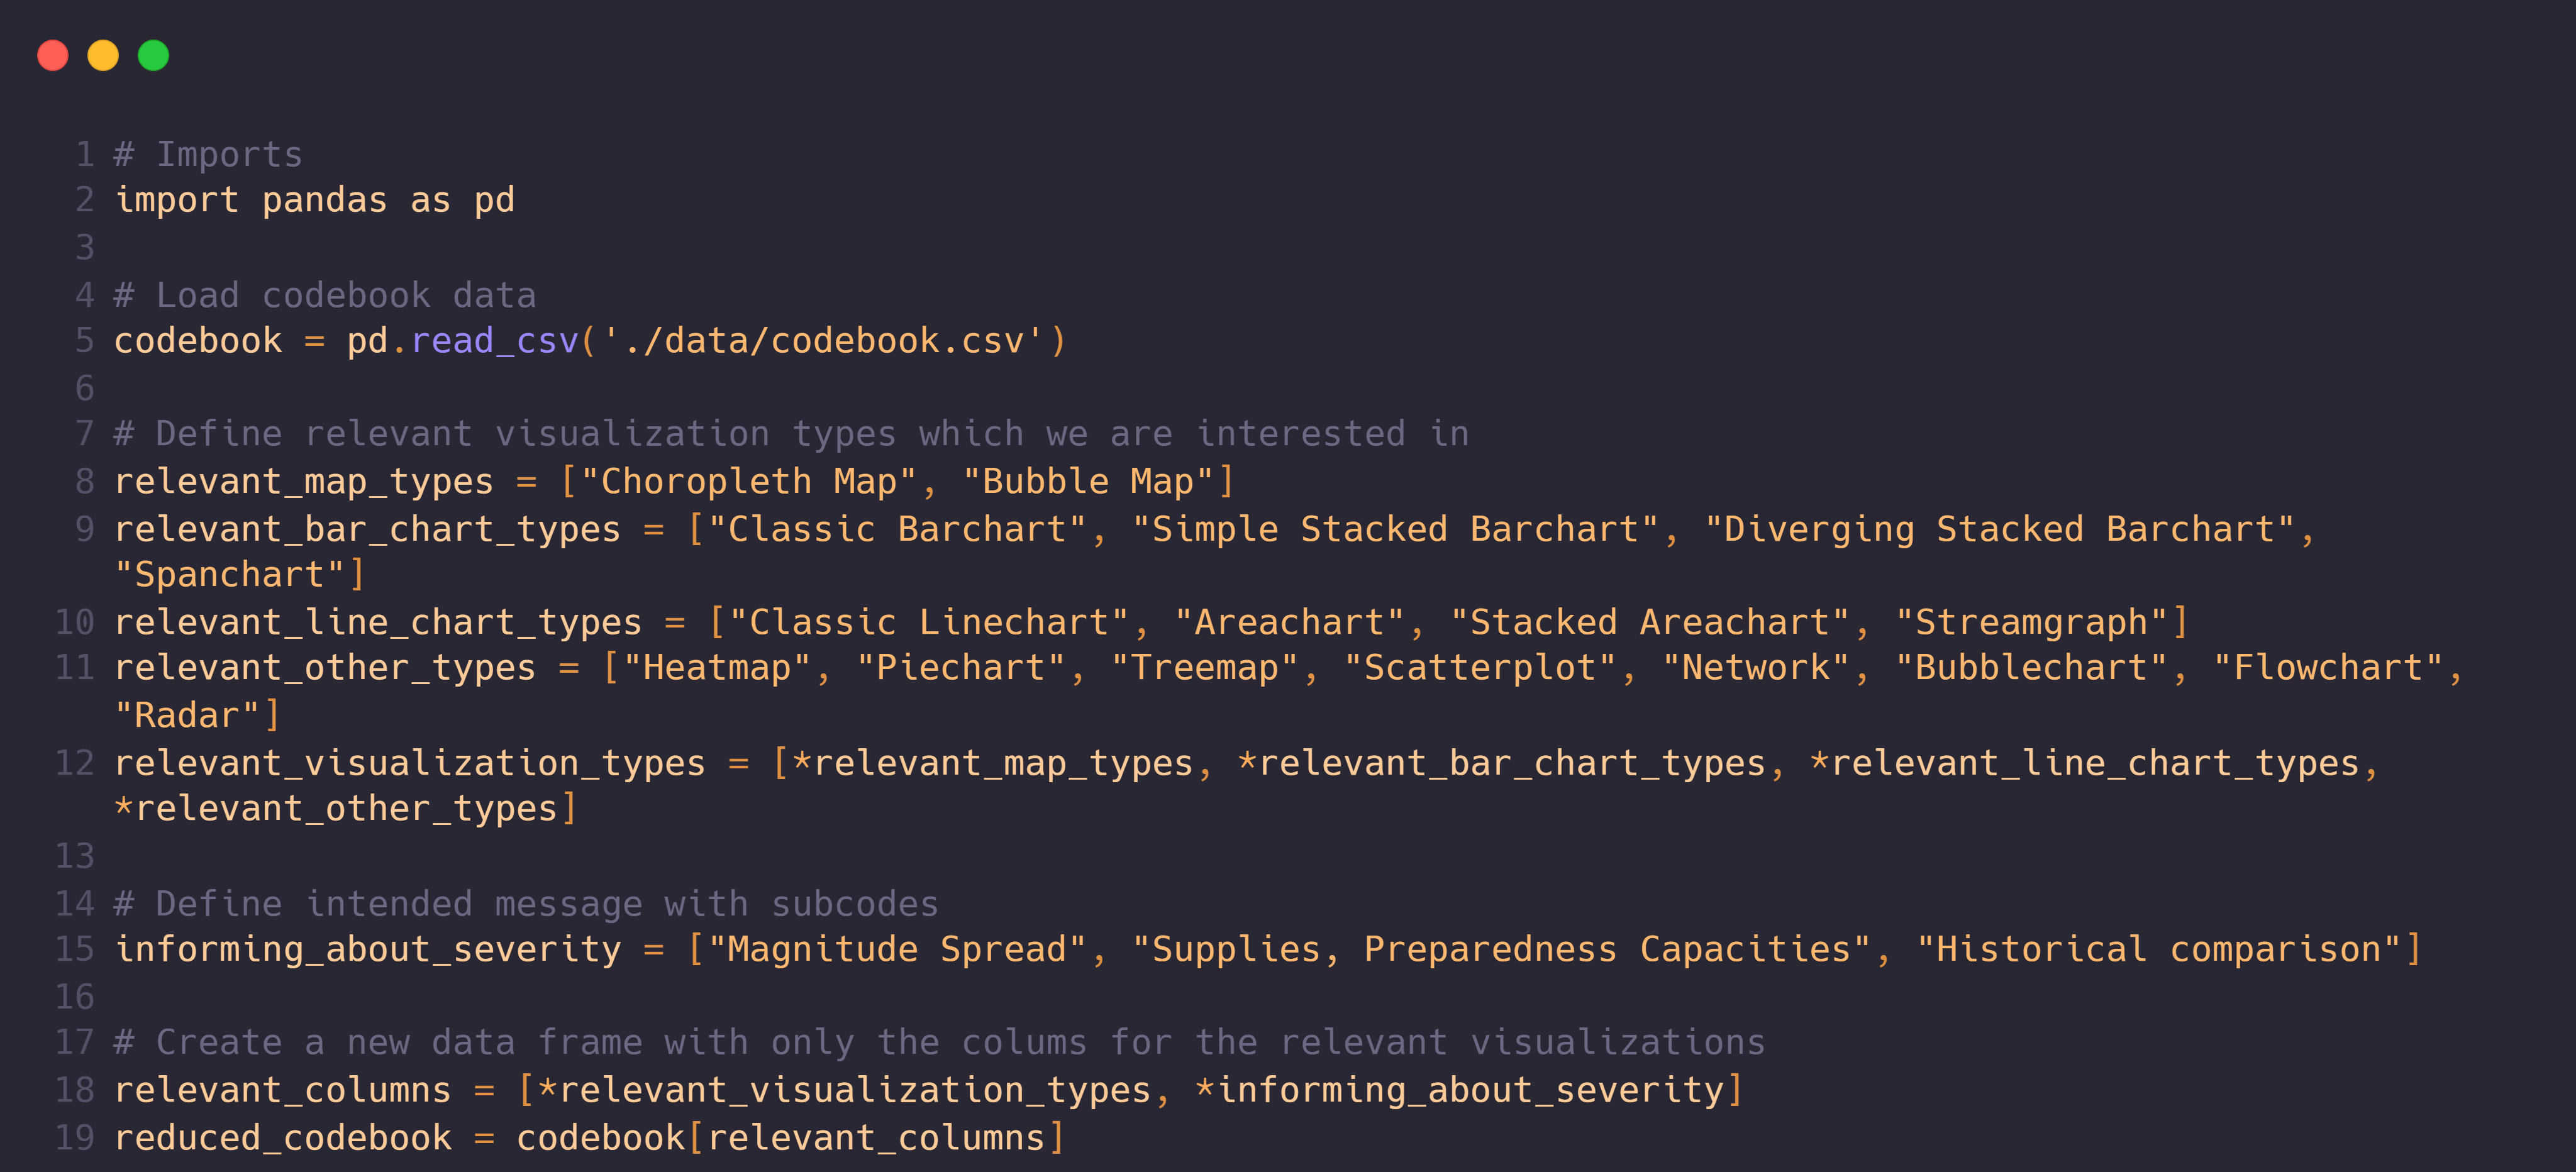
\includegraphics[width=14cm]{images/jupyter_notebook_data_reduction.png}
    \centering
    \caption{Datenreduktion des Codebooks mithilfe von Jupyter Notebook (Eigene Darstellung)}
    \label{fig:jupyter_notebook_data_reduction}
\end{figure}

\clearpage
\noindent
\textbf{Filterung der Daten nach Kategorie}
\newline
\indent
Zhang definierte pro Kategorie entsprechende Subkategorien. ``Magnitude Spread`` ist beispielsweise eine Subkategorie, welche zur Hauptkategorie ``Informing of the Severity gehört`` (siehe Abbildung \ref{fig:zhang_codebook_intended_message}). Pro Zeileneintrag im Codebook ist somit definiert, zu welchen Subkategorien der Eintrag gehört. Jedoch müssen für eine Übersicht der Datenvisualisierungen \textbf{pro Kategorie} die Daten noch entsprechend gruppiert werden. Um dies zu bewerkstelligen wurde jeder Zeileneintrag ausgewertet und geschaut ob er einen Wahrheitswert von True in den entsprechenden Subkategorien beinhaltet. Falls also ein Eintrag mindestens ein Wahrheitswert in den relevanten Subkategorien aufweist, wurde er der entsprechenden Hauptkategorie zugeordnet. Zeile 2 in Abbildung \ref{fig:jupyter_notebook_data_filtering} identifiziert ob eine Zeile zu einer bestimmten Kategorie gehört, ist dies der Fahl wird für diese Zeile der Wahrheitswert \textbf{True} hinterlegt.
Anschliessend wird in Zeile 3 das Codebook gefiltert. Hierbei wird jede Zeile durchgegangen und überprüft, ob diese Zeile einen Wahrheitswert von True hat. Somit sind die Daten nun nach der gewünschten Kategorie gefiltert.


 \begin{figure}[h]
    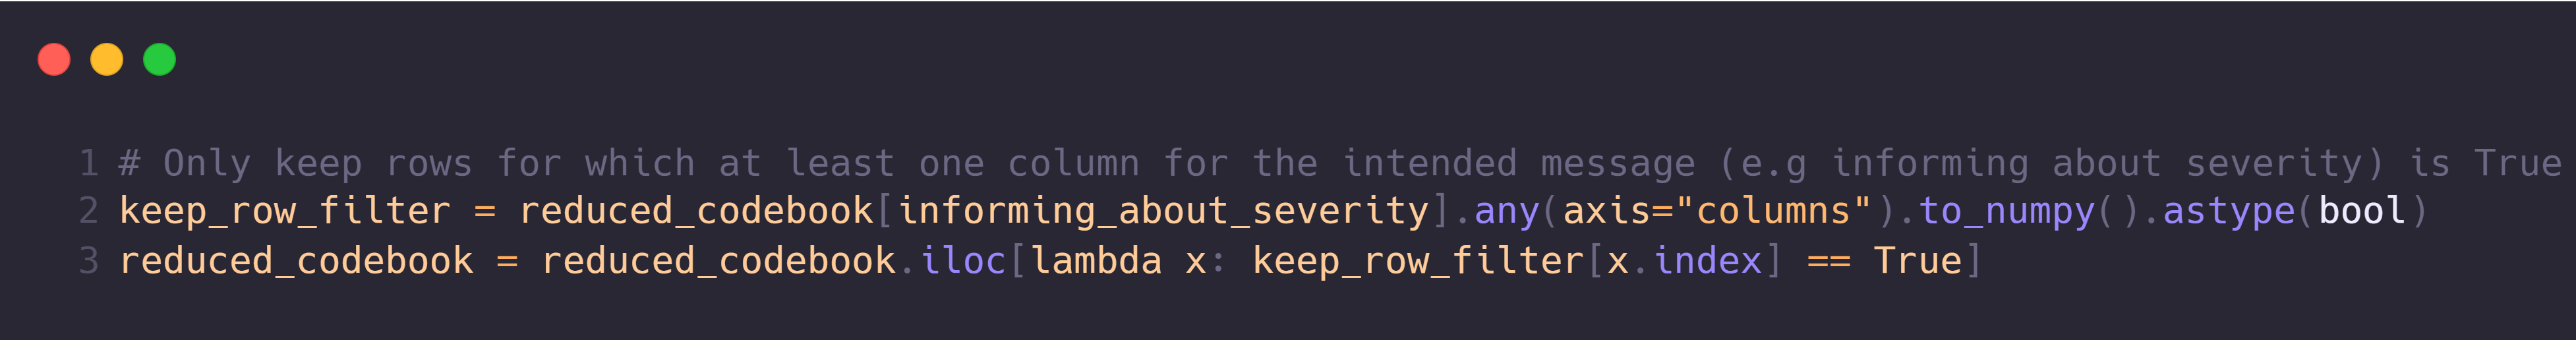
\includegraphics[width=14cm]{images/jupyter_notebook_data_filtering.png}
    \centering
    \caption{Ermittlung welche Zeilen des Codebooks zu den entsprechenden Kategorien gehören (Eigene Darstellung)}
    \label{fig:jupyter_notebook_data_filtering}
\end{figure}


\noindent
\textbf{Filterung der Daten nach einer bestimmten Subkategorie}
\newline
\indent
Im Gegensatz zur Filterung der Daten nach einer bestimmten Kategorie (welche mehrere Subkategorien beinhaltet), ist die Filtetrung nach einer bestimmten Subkategorie einfacher. Auf Zeile 2 in Abbildung \ref{fig:jupyter_notebook_data_filtering_subcategory} wird die Subkategorie, nach welcher gefiltert werden soll definiert. Anschliessend wird jede Zeile durchgegangen und überprüft ob für diese Subkategorie einen Wahrheitswert von True existiert (siehe Zeile 9 in Abbildung \ref{fig:jupyter_notebook_data_filtering_subcategory}).


 \begin{figure}[h]
    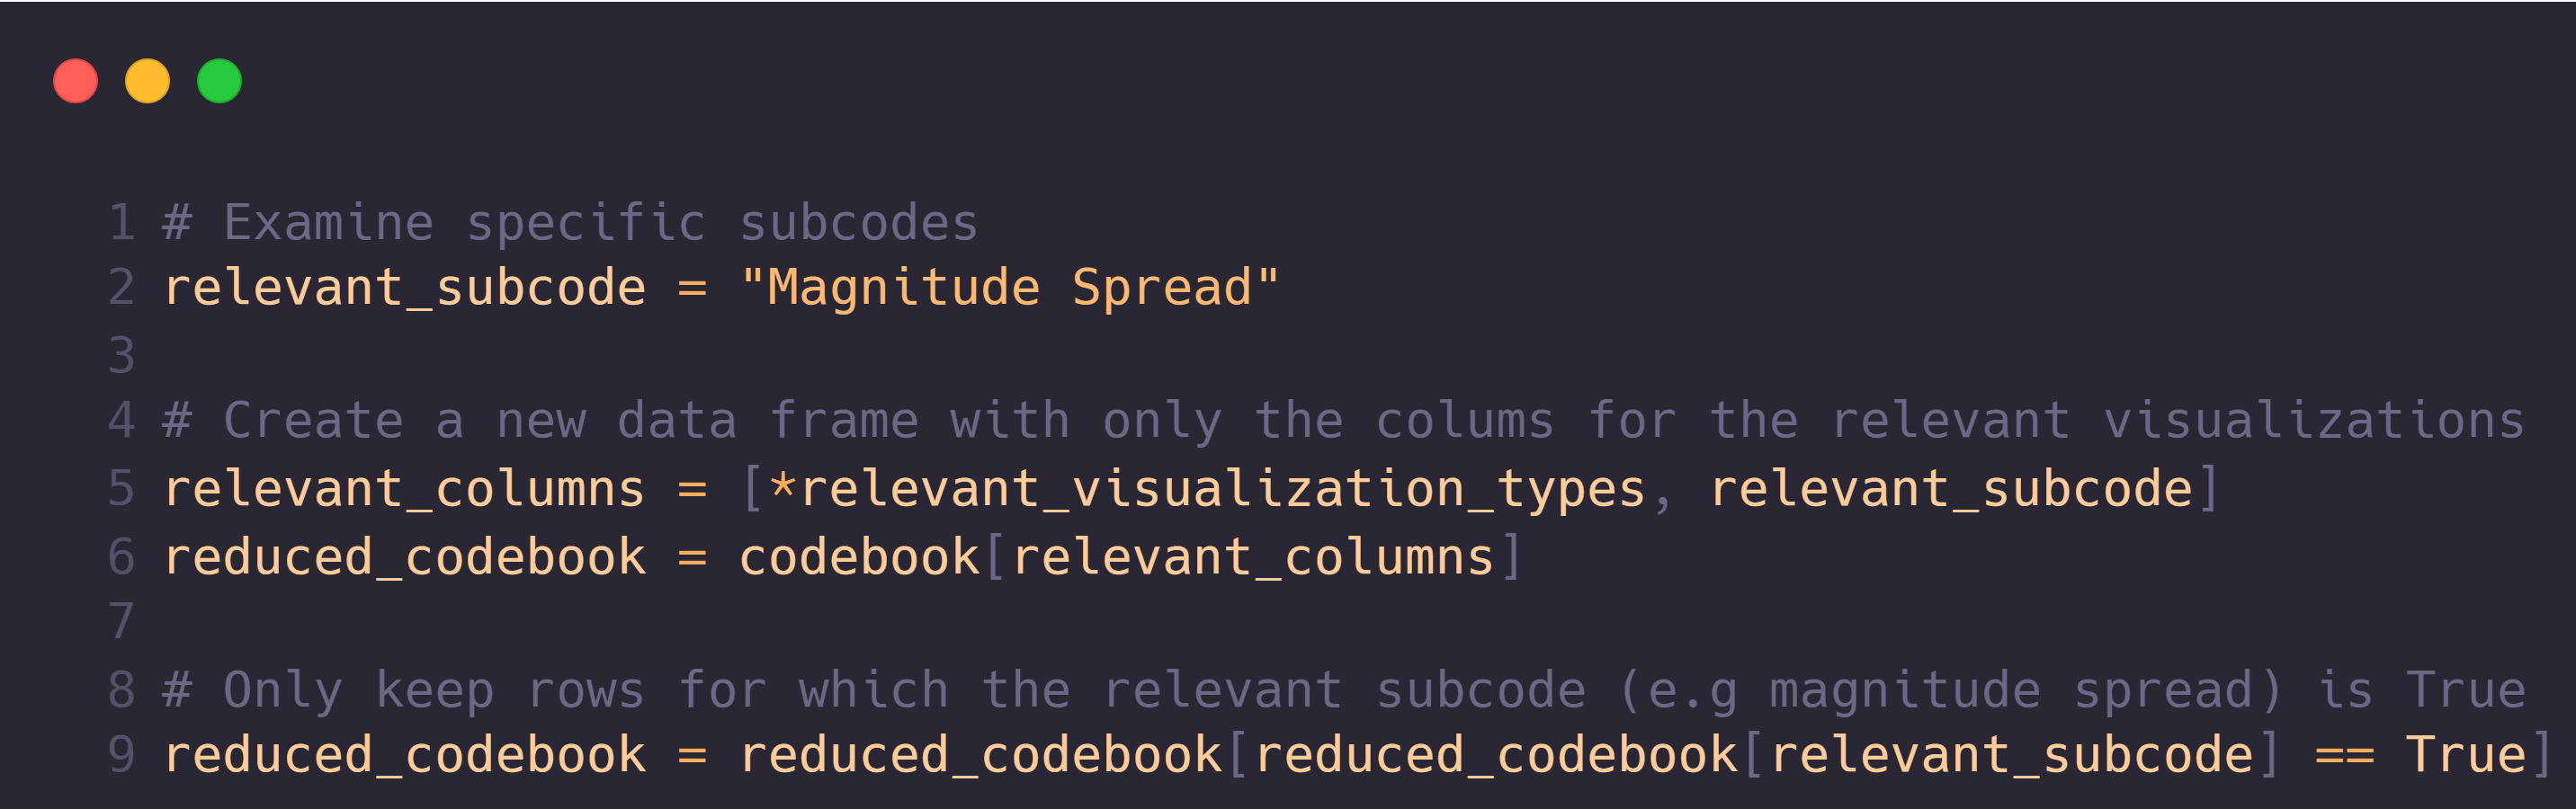
\includegraphics[width=14cm]{images/jupyter_notebook_data_filtering_subcategory.png}
    \centering
    \caption{Filterung des Codebooks nach einer bestimmten Subkategorie (Eigene Darstellung)}
    \label{fig:jupyter_notebook_data_filtering_subcategory}
\end{figure}

\clearpage
\noindent
\textbf{Visualisierung der Daten}
\newline
\indent
Die reduzierten und gefilterten Daten müssen noch visualisiert werden. Hierzu wurden für jede relevante Datenvisualisierung durchgegangen und ermittelt wie viel Mal diese Visualisierung mit dem Wert True auftrat (siehe Zeile 4-7 in Abbildung \ref{fig:jupyter_notebook_data_visualization}).


\begin{figure}[h]
    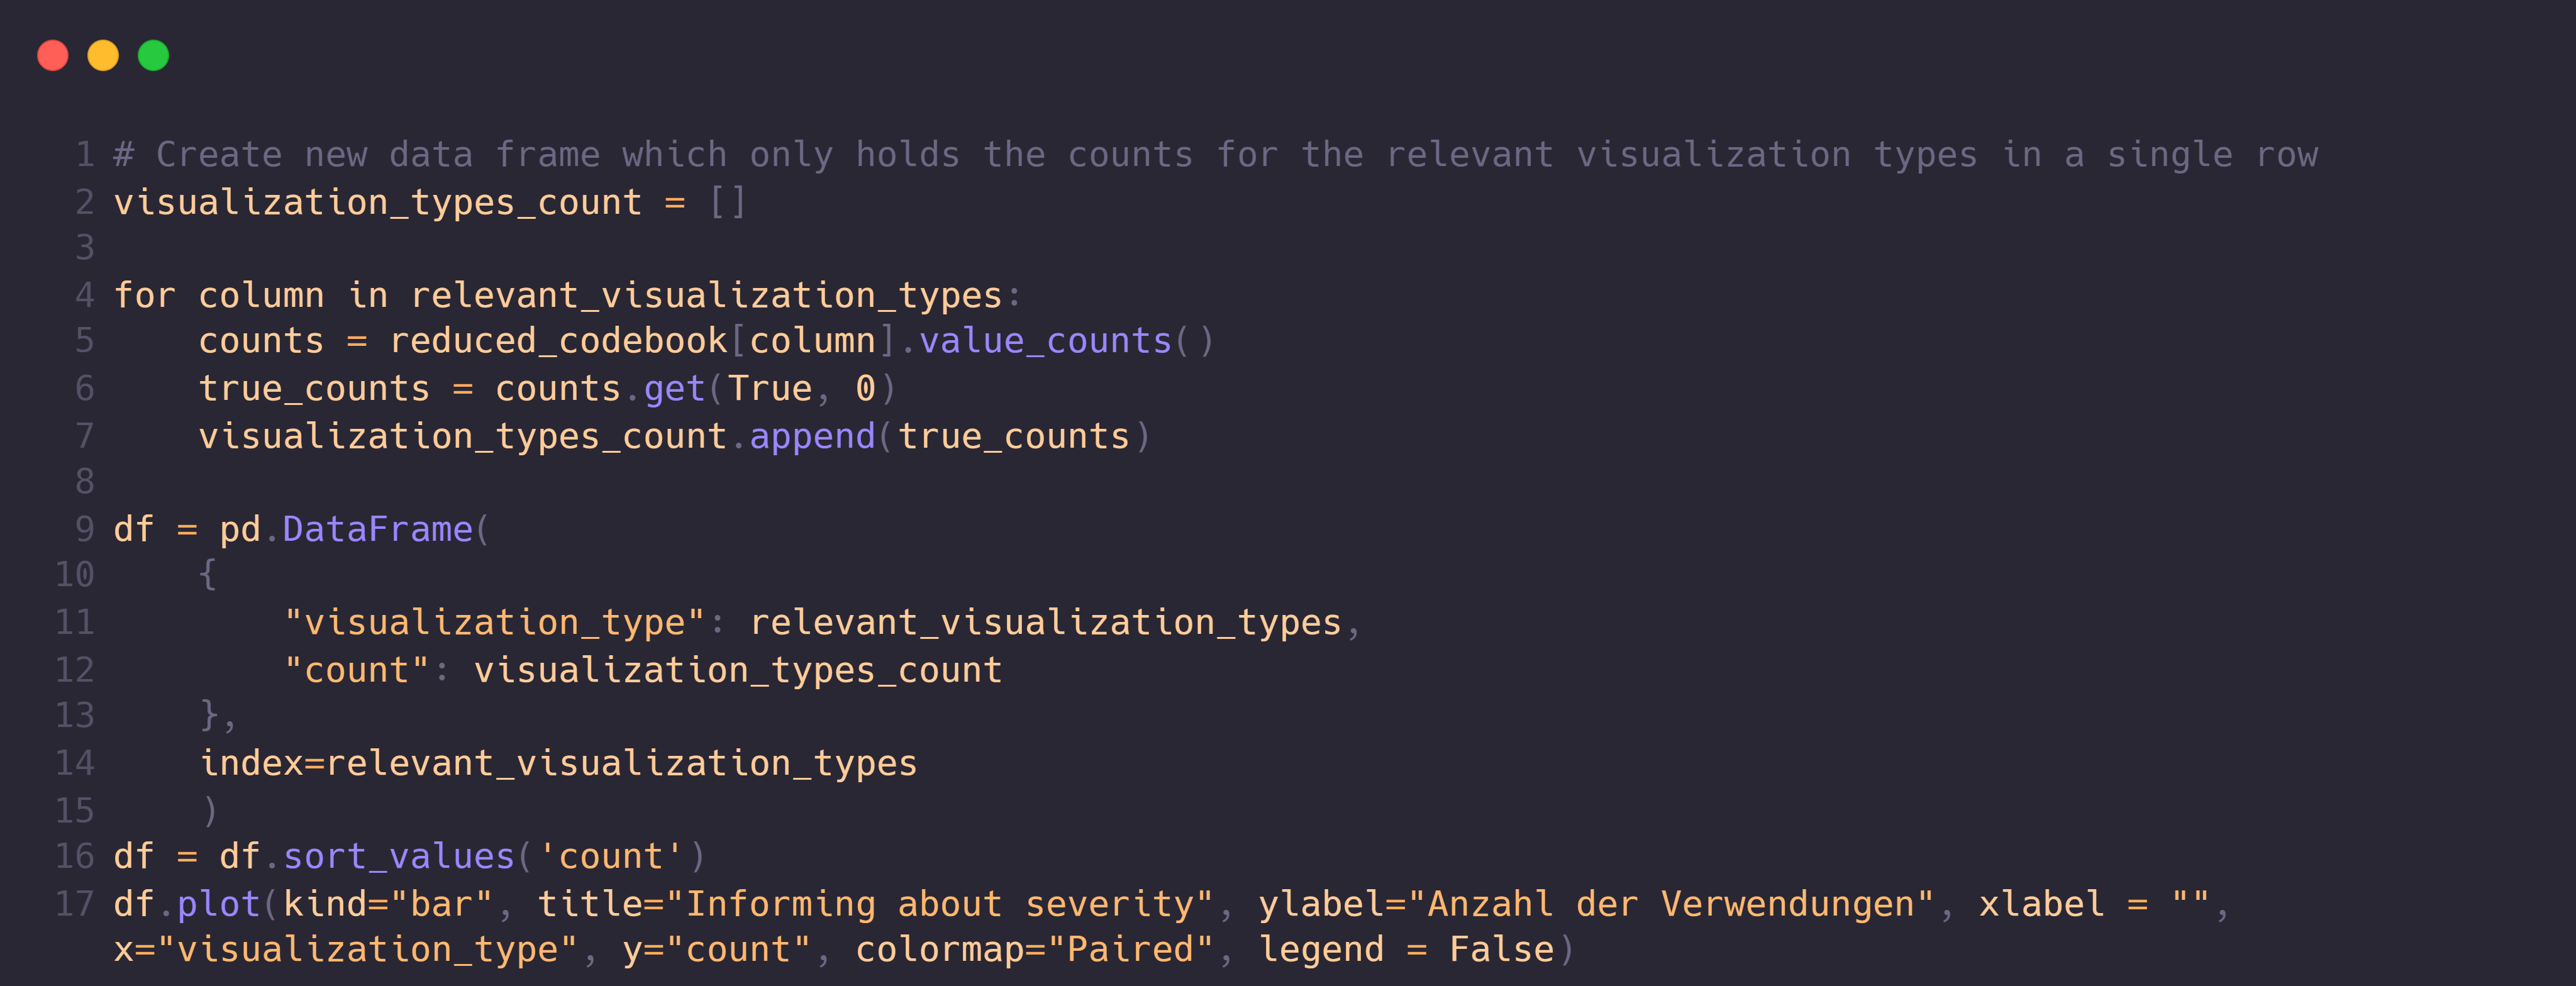
\includegraphics[width=14cm]{images/jupyter_notebook_data_visualization.png}
    \centering
    \caption{Darstellung der aufbereiteten Daten aus dem Codebook (Eigene Darstellung)}
    \label{fig:jupyter_notebook_data_visualization}
\end{figure}

Anschliessend wurde das Ergebnis als Balkendiagramm mit Hilfe der \textbf{plotly} Bibliothek dargestellt (siehe Abbildung \ref{fig:plotly_data_visualization_per_category}).

 \begin{figure}[h]
    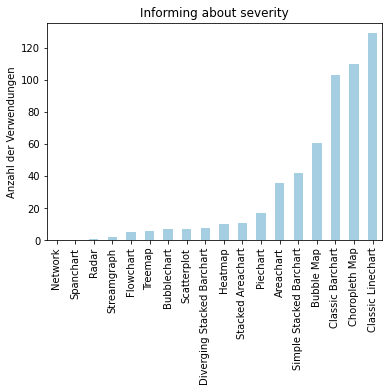
\includegraphics[width=10cm]{images/plotly_data_visualization_per_category.png}
    \centering
    \caption{Visualisierung der aufbereiteten Daten als Balkendiagramm (Eigene Darstellung)}
    \label{fig:plotly_data_visualization_per_category}
\end{figure}


\clearpage
\noindent
\textbf{Auswertung der Daten}
\newline
\indent
Diese Methodik wurde für die restlichen Kategorien sowie Subkategorien wiederholt. Tabelle \ref{table:jupyter_notebook_most_used_data_visualizations_per_category} zeigt die vier am meisten verwendeten Datenvisualisierungen pro Kategorie auf. Die Ergebnisse sind hierbei nach der Häufigkeit der Verwendung von Links nach Rechts sortiert.

% Begin Table Most used Data Visualizations per Category
\begin{table}[h]
\centering
\resizebox{\textwidth}{!}{%
\begin{tabular}{@{}ll@{}}
\toprule
\textbf{Kategorie} & \textbf{Meist verwendete Datenvisualisierungen sortiert von Links nach Rechts} \\ \midrule
Informing about severity & Classic Linechart, Choropleth Map, Classic Barchart, Bubble Map \\ \midrule
Forecasting Trends and Influences & Classic Linechart, Choropleth Map, Classic Barchart, Simple Stacked Barchart \\ \midrule
Gauging the multifaceted impact of the crisis & Classic Linechart, Classic Barchart, Choropleth Map, Simple Stacked Barchart \\ \midrule
Examining the Nature of the Crisis & Classic Linechart, Classic Barchart, Choropleth Map, Flowchart \\ \midrule
Guiding Risk mitigation & Classic Linechart, Areachart, Simple Stacked Barchart, Classic Barchart \\ \midrule
Communicating risk, vulnerability and equity & Choropleth Map, Classic Linechart, Classic Barchart, Bubble Map \\ \bottomrule
\end{tabular}
}
\caption{Top 4 am meisten verwendeten Datenvisualisierung pro Kategorie (Eigene Darstellung)}
\label{table:jupyter_notebook_most_used_data_visualizations_per_category}
\end{table}
% End Table Most used Data Visualizations per Category

Zusätzlich war mit dem obenen beschriebenen Vorgehen auch eine Aufschlüsselung nach Subkategorie möglich (siehe Abbildung \ref{fig:jupyter_notebook_data_filtering_subcategory}). Tabelle \ref{table:jupyter_notebook_most_used_data_visualizations_per_subcategory} veranschaulicht die vier am meisten verwendeten Datenvisualisierungen heruntergebrochen auf die Subkategorie.

% Begin Table Data Visualizations per Subcategory
\begin{table}[h]
\centering
\resizebox{\textwidth}{!}{%
\begin{tabular}{@{}ll@{}}
\toprule
\textbf{Subkategorie} & \textbf{Meist verwendete Datenvisualisierungen} \\ \midrule
Magnitude Spread & Classic Linechart, Choropleth Map, Classic Barchart, Bubble Map \\ \midrule
Supplies, Prepardness, Capacities & Choropleth Map,  Classic Barchart, Classic Linechart, Bubble Map \\ \midrule
Historical comparison & Classic Linechart, Classic Barchart, Bubble Map, Treemap \\ \midrule
R-Naught & Classic Linechart, Choropleth Map, Simple Stacked Barchart, Classic Barchart \\ \midrule
Projection of numbers & Classic Linechart, Choropleth Map, Classic Barchart, Simple Stacked Barchart \\ \midrule
Economic & Classic Linechart, Classic Barchart, Simple Stacked Barchart, Choropleth Map \\ \midrule
Social & Classic Linechart, Choropleth Map, Classic Barchart, Scatterplot \\ \midrule
Environmental & Classic Linechart, Choropleth Map, Classic Barchart, Heatmap \\ \midrule
Political & Classic Linechart, Choropleth Map, Classic Barchart, Bubble Map \\ \midrule
Policy Order Intervention Related & Classic Linechart, Classic Barchart, Scatterplot, Choropleth Map \\ \midrule
Explain the nature of the crisis in general & Classic Linechart, Classic Barchart, Choropleth Map, Flowchart \\ \midrule
Explain Coronavirus & Choropleth Map, Classic Linechart, Areachart, Bubble Map \\ \midrule
Map symptoms, diagnosis, treatment & Classic Barchart, Classic Linechart, Bubble Map, Choropleth Map \\ \midrule
Explain transimission  \& reasonableness of intervention & Classic Linechart, Classic Barchart, Choropleth Map, Bubble Map \\ \midrule
Contact Tracing & Flowchart, Classic Barchart, Classic Linechart, Bubble Map \\ \midrule
Social Distancing & Simple Stacked Barchart, Classic Linechart, Classic Barchart, Areachart \\ \midrule
PPE & Scatterplot, Radar, Bubblechart, Bubble Map \\ \midrule
Hygiene & Bubble Map, Classic Linechart, Flowchart, Classic Barchart \\ \midrule
Flatten the Curve & Classic Linechart, Areachart, Classic Barchart, Choropleth Map \\ \midrule
Communicating risk, vulnerability and equity & Choropleth Map, Classic Linechart, Classic Barchart, Bubble Map \\ \bottomrule
\end{tabular}%
}
\caption{Top 4 am meisten verwendeten Datenvisualisierung pro Subkategorie (Eigene Darstellung)}
\label{table:jupyter_notebook_most_used_data_visualizations_per_subcategory}
\end{table}
% End Table Data Visualizations per Subcategory

\clearpage
\subsubsection{Identifizierung von Awendungsfällen} \label{ch:identification_of_use_cases}
Eine Datenvisualisierung alleine reicht nicht aus, sie benötigt einen Anwendungsfall um verstanden zu werden. In einem nächsten Schritt sind daher Anwendungsfälle identifiziert worden. Als Kontext für die Definition der Anwendungsfälle sind hierbei die identifizierten Subkategorien von Zhang verwendet worden. Tabelle \ref{table:match_subcategories_to_categories} zeigt hierbei die Zuordnung der Subkateogrien zu den entsprechenden Kategorien. Die Definitionen von Zhang sind hierbei in Klammern beigefügt.

% Start Table Matching Subcategory to Categories
\begin{table}[h]
\centering
\resizebox{\textwidth}{!}{%
\begin{tabular}{@{}ll@{}}
\toprule
\textbf{Kategorie} & \textbf{Subkategorien} \\ \midrule
\begin{tabular}[c]{@{}l@{}}Informationen über den Schweregrad der Pandemie\\ (Informing of the serverity)\end{tabular} & \begin{tabular}[c]{@{}l@{}}Informationen über Corona Fallzahlen (Magnitude Spread)\\ Informationen über Spitalauslastungen (Supplies, Prepardness, Capacities)\\ Historische Vergleiche mit anderen Pandemien (Historical comparison)\end{tabular} \\ \midrule
\begin{tabular}[c]{@{}l@{}}Trendvorhersagen zu Corona\\ (Forecasting trends and influences)\end{tabular} & \begin{tabular}[c]{@{}l@{}}Vorhersagen über Ansteckungszahlen (R-Naught)\\ Vorhersagen über Todesfälle (Projectsions of numbers)\end{tabular} \\ \midrule
\begin{tabular}[c]{@{}l@{}}Einfluss der Pandemie\\ (Gauging the multifaceted impact of the crisis)\end{tabular} & \begin{tabular}[c]{@{}l@{}}Einfluss auf Ökonomie (Economic)\\ Einfluss auf das Soziale Gefüge (Social)\\ Einfluss auf die Umwelt (Environmental)\\ Einfluss auf die Politik (Political impact)\\ Einfluss aufgrund einer rechtlichen Vorschrift (Policy Order Intervention Related)\end{tabular} \\ \midrule
\begin{tabular}[c]{@{}l@{}}Erklärung der Natur des Corona Virus\\ (Examining the nature of the crisis)\end{tabular} & \begin{tabular}[c]{@{}l@{}}Erklärungen zum Coronavirus im Allgemeinen (Explain coronavirus)\\ Erklärungen zu Symptomen, Diagnosen und Behandlungen (Map symptoms, diagnosis, treatment)\\ Erklärungen zur Übertragung des Corona Virus (Explain transmission)\\ Contact Tracing (Contact Tracing)\end{tabular} \\ \midrule
\begin{tabular}[c]{@{}l@{}}Risikoverminderung des Corona Virus\\ (Guiding risk mitigation)\end{tabular} & \begin{tabular}[c]{@{}l@{}}Social Distancing (Social Distancing)\\ Informationen über Schutzequipment (PPE)\\ Informationen über Hygiene (Hygiene)\\ Informationen um die Corona Kurve flach zu halten (Flatten the Curve)\end{tabular} \\ \midrule
\begin{tabular}[c]{@{}l@{}}Informationen über die Verletzlichkeit bestimmter Personen\\ (Communicating risk, vulnerability, and equity)\end{tabular} & \begin{tabular}[c]{@{}l@{}}Informationen zu Personen in einem bestimmten Alter\\ Informationen zu Personen eines bestimmten Geschlechts\\ Informationen zu Personen einer bestimmten Nationalität\end{tabular} \\ \bottomrule
\end{tabular}
}
\caption{Zuordnung der Subkategorien zu den entsprechenden Kategorien (Eigene Darstellung in Anlehnung auf Abbildung \ref{fig:zhang_codebook_intended_message})}
\label{table:match_subcategories_to_categories}
\end{table}
% End Table Matching Subcategory to Categories


\noindent
\textbf{Anwendungsfälle im Bereich ``Schweregrad der Pandemie``}
\newline
\indent
Sowohl die Corona Fallzahlen als auch die Spitalauslastungen sind bereits spezifische Anwendungsfälle. Für den historischen Vergleich mit anderen Pandemien wurde als Anwendungsfall der Vergleich mit Pandemien in Bezug auf die Ansteckungszahlen definiert. Tabelle \ref{table:use_cases_for_severity_of_pandemic} zeigt die definierten Anwendungsfälle auf die jeweiligen Subkategorien auf.

% Begin Table Use cases in category Severity of Pandemic
\begin{table}[h]
\centering
\resizebox{\textwidth}{!}{%
\begin{tabular}{@{}ll@{}}
\toprule
\textbf{Subkategorie} & \textbf{Anwendungsfall} \\ \midrule
Informationen über Corona Fallzahlen & Corona Fallzahlen darstellen \\ \midrule
Informationen über Spitalauslastungen & Spitalauslastungen darstellen \\ \midrule
Historische Vergleiche mit anderen Pandemien & Vergleich mit anderen Pandemien in Bezug auf die Ansteckungszahlen \\ \bottomrule
\end{tabular}
}
\caption{Zuordnung der Anwendungsfälle für die Kategorie ``Schweregrad der Pandemie`` (Eigene Darstellung)}
\label{table:use_cases_for_severity_of_pandemic}
\end{table}
% End Table Use cases in category Severity of Pandemic

\clearpage
\noindent
\textbf{Anwendungsfälle im Bereich ``Trendvorhersagen zu Corona``}
\newline
\indent
In diesem Bereich wurden direkt die definierten Subkategorien aus Tabelle \ref{table:match_subcategories_to_categories} als Anwendungsfälle übernommen (siehe Tabelle \ref{table:use_cases_for_forecast_of_pandemic}).

% Begin Table Use cases in category Forecast of Pandemic
\begin{table}[h]
\centering
\resizebox{\textwidth}{!}{%
\begin{tabular}{@{}ll@{}}
\toprule
\textbf{Subkategorie} & \textbf{Anwendungsfall} \\ \midrule
Vorhersagen über Ansteckungszahlen & Vorhersagen über Ansteckungszahlen \\ \midrule
Vorhersagen über Todesfälle & Vorhersage über Todesfälle \\ \bottomrule
\end{tabular}%
}
\caption{Zuordnung der Anwendungsfälle für die Kategorie ``Trendvorhersagen zu Corona`` (Eigene Darstellung)}
\label{table:use_cases_for_forecast_of_pandemic}
\end{table}
% End Table Use cases in category Forecast of Pandemic

\noindent
\textbf{Anwendungsfälle im Bereich ``Einfluss der Pandemie``}
\newline
\indent
Die Subkategorien im Bereich ``Einfluss der Pandemie`` sind sehr allgemein gehalten (Ökonomie, Politik etc.). Mithilfe der Sonderseite vom \gls{bfs} in Bezug auf Corona, war es jedoch möglich für einen Grossteil der identifizierten Bereiche einen Anwendungsfall zu finden ~\citep{bfs_covid19_page}. Für den Bereich der Politik wurden die Anzahl der Abstimmungen in Bezug auf Covid relevante Gesetze als Anwendungsfall identifiziert. Für den Einfluss von rechtlichen Vorschriften wurde der Effekt des Corona Lockdowns auf die Fallzahlen verwendet. Tabelle \ref{table:use_cases_for_influence_of_pandemic} zeigt die identifizierten Anwendungsbereiche in Bezug auf den Einluss der Pandemie nochmals auf.

% Begin Table Use cases in category Influence of Pandemic
\begin{table}[h]
\centering
\resizebox{\textwidth}{!}{%
\begin{tabular}{@{}ll@{}}
\toprule
\textbf{Subkategorie} & \textbf{Anwendungsfall} \\ \midrule
Einfluss auf Ökonomie & Einfluss von Corona auf Umsatzzahlen im IT-Sektor \\ \midrule
Einfluss auf das Soziale Gefüge & Anzahl Personen aufzeigen, welche soziale Unterstützung aufgrund Corona beziehen \\ \midrule
Einfluss auf die Umwelt & Einfluss von Corona auf die Anzahl der Flüge im Luftverkehr \\ \midrule
Einfluss auf die Politik & Anzahl der Abstimmungen zu einem politischen Thema in Bezug auf Corona \\ \midrule
Einfluss aufgrund einer rechtlichen Vorschrift & Einfluss des Corona Lockdowns auf die Fallzahlen \\ \bottomrule
\end{tabular}%
}
\caption{Zuordnung der Anwendungsfälle für die Kategorie ``Einfluss der Pandemie`` (Eigene Darstellung)}
\label{table:use_cases_for_influence_of_pandemic}
\end{table}
% End Table Use cases in category Influence of Pandemic

\noindent
\textbf{Anwendungsfälle im Bereich ``Erklärung der Natur des Corona Virus``}
\newline
\indent
Für Erklärungen zum Coronavirus im Allgemeinen wurde der Anwendungsfall explizit so belassen, um herausfinden zu können, welche Datenvisualisierung jenseits der bereits identifizierten Visualisierungen durch das Jupyter Notebook (siehe Tabelle \ref{table:jupyter_notebook_most_used_data_visualizations_per_subcategory}), der Nutzer für diesen Zweck verwenden würde. In Bezug auf Symptome, Diagnosen sowie Behandlungen ist es interessant herauszufinden, wie viel Prozent der Bevölkerung die vom Bund vorgeschriebenen Schutzmassnahmen (siehe Abbildung \ref{fig:bag_infographic}) bereits umsetzen. Für die Übertragung des Corona Virus sind die Übertragungswege eine wichtige Information. Eine stark verbeitete App in Bezug auf das Contact Tracing in der Schweiz ist SwissCovid. In diesem Zusammenhang sind die Anzahl der eingereichten Covid Codes interessant. Die identifizierten Szenarien sind in Tabelle \ref{table:use_cases_for_nature_of_covid} ersichtlich.

% Begin Table Uses Cases for Explaining Nature of Covid
\begin{table}[]
\centering
\resizebox{\textwidth}{!}{%
\begin{tabular}{@{}ll@{}}
\toprule
\textbf{Subkategorie} & \textbf{Anwendungsfall} \\ \midrule
Erklärungen zum Coronavirus im Allgemeinen & Erklärungen zum Coronavirus im Allgemeinen \\ \midrule
Erklärungen zu Symtpomen, Diagnose und Behandlungen & Wie viel Prozent der Bevölkerung setzen die Corona Schutzmassnahmen bereits um \\ \midrule
Erklärungen zur Übertragung des Corona Virus & Über welche Wege (Hände schütteln etc.) das Virus am meisten übetragen wird \\ \midrule
Contact Tracing & Anzahl eingereichter Covid Codes via SwissCovid \\ \bottomrule
\end{tabular}%
}
\caption{Zuordnung der Anwendungsfälle für die Kategorie ``Erklärung der Natur des Corona Virus`` (Eigene Darstellung)}
\label{table:use_cases_for_nature_of_covid}
\end{table}
% End Table Uses Cases for Explaining Nature of Covid

\noindent
\textbf{Anwendungsfälle im Bereich ``Risikoverminderung des Corona Virus``}
\newline
\indent
Für Social Distancing ist eine Datenvisualisierung welche aufzeigt, wie hoch die Gefahr einer Ansteckung abhängig von der Anzahl der Personen in der unmittelbaren Umgebung ist, interessant. Ein weit verbreitetes Schutzequipment in Zeiten der Corona Pandemie sind Schutzmasken. Aufgrund dessen ist es interessant den Wirkungsgrad von Masken zu untersuchen. Gleichermassen ist die Wirksamkeit von Hygienemassnahmen auf Fallzahlen in der Kategorie ``Hygiene`` von Interesse.
Für die Kategorie ``Informationen um die Corona Kurve flach zu halten`` wurde aufgrund der vielen Einflussfaktoren entschieden, keinen Anwendungsfall zu definierten (siehe Tabelle \ref{table:use_cases_risk_mitigation}).

% Begin Table Use Cases for Risk Mitigation
\begin{table}[h]
\centering
\resizebox{\textwidth}{!}{%
\begin{tabular}{@{}ll@{}}
\toprule
\textbf{Subkategorie} & \textbf{Anwendungsfall} \\ \midrule
Social Distancing & Gefahr einer Ansteckung abhängig von der Anzahl der Personen in der unmittelbaren Umgebung \\ \midrule
Informationen zu Schutzequipment & Wirksamkeit von Schutzmasken \\ \midrule
Informationen über Hygiene & Wirksamkeit von Hygienemassnahmen auf Corona Fallzahlen \\ \midrule
Informationen um die Corona Kurve flach zu halten & - \\ \bottomrule
\end{tabular}%
}
\caption{Zuordnung der Anwendungsfälle für die Kategorie ``Risikoverminderung des Corona Virus`` (Eigene Darstellung)}
\label{table:use_cases_risk_mitigation}
\end{table}
% End Table Use Cases for Risk Mitigation

\noindent
\textbf{Anwendungsfälle im Bereich ``Informationen über die Verletzlichkeit bestimmter Personen``}
\newline
\indent
Die Kategorie ``Communicating risk, vulnerability, and equity`` hat gemäss dem Codebook von Zhang keine Subkategorien. Jedoch wurden im Rahmen dieser Arbeit die Verletzlichkeit bestimmter Personengruppen in Bezug auf die Faktoren Alter, Geschlecht sowie Nationalität definiert. Konkret sollen hierbei die Fallzahlen untersucht werden (siehe Tabelle \ref{table:use_cases_vulnerability}).

% Begin Table Use Cases Vulnerability of people
\begin{table}[h]
\centering
\resizebox{\textwidth}{!}{%
\begin{tabular}{@{}ll@{}}
\toprule
\textbf{Subkategorie} & \textbf{Anwendungsfall} \\ \midrule
Informationen zu Personen in einem bestimmten Alter & Corona Fallzahlen innerhalb von verschiedenen Altersgruppen \\ \midrule
Informationen zu Personen eines bestimmten Geschlechts & Corona Fallzahlen innerhalb von verschiedenen Geschlechtern \\ \midrule
Informationen zu Personen einer bestimmten Nationalität & Corona Fallzahlen nach verschiedenen Geschlechtern \\ \bottomrule
\end{tabular}%
}
\caption{Zuordnung der Anwendungsfälle für die Kategorie ``Informationen über die Verletzlichkeit bestimmter Personen`` (Eigene Darstellung)}
\label{table:use_cases_vulnerability}
\end{table}
% End Table Use Cases Vulnerability of people

\subsubsection{Erstellung des Online Fragebogens}
Mithilfe der identifizierten Datenvisualisierungen pro Subkategorie sowie den dazugehörigen Anwendungsfällen wurde ein Online Fragebogen\footnote{https://forms.gle/9hMHiRaQLPuDC2Wo8} mit Hilfe von Google Forms, welches eine automatische Auswertung der Ergebnisse erlaubt, erstellt. Der erstellte Fragebogen soll als Grundlage dienen um sowohl die untergeordnete Forschungsfrage 1 (Welche \textbf{Visualisierungsarten} in Bezug auf Corona werden von Millennials gefordert?) sowie untergeordnete Forschungsfrage 2 (Welche \textbf{Informationen} in Bezug auf Corona werden von Millennials gefordert?) zu beantworten. Als Grundlage für die Informationsermittlung werden hierbei die identifizierten Kategorien sowie Subkategorien von Zhang verwendet (siehe Kapitel \ref{ch:analysis_of_codebook}). Für die Ermittlung der Visualisierungen werden die identifizierten Visualisierungen in Kombination mit den Anwendungsfällen verwendet (siehe Kapitel \ref{ch:identification_of_use_cases}).\\

\subsubsection{Erstellung des Interviewleitfadens} \label{ch:creation_of_interview_guide}
Um zusätzliche Informationen in Bezug auf Corona Datenvisualisierungen sowie gewünschte Personalisierungsmöglichkeite der Zielgruppe Millennials zu erhalten wurde beschlossen, nebst dem Online Fragebogen, ein Interview durchzuführen.
Im Rahmen des Interviews, soll das Corona Dashboard der Schweiz\footnote{https://www.covid19.admin.ch/de/overview} besucht und erforscht werden. Anschliessend soll mit Hilfe des \textbf{think-aloud} (lautes Denken) Ansatzes die wichtigsten Gedanken festgehalten werden.\\

\noindent
\textbf{Grundlegende Informationen zum Dashboard}
\newline
\indent
In einem ersten Schritt sollen dabei grundlegende Informationen zum Dashboard abgeholt werden. Ähnlich wie bei einer Scrum Retrospektive soll dabei festgehalten werden, was den Probanden besonders am Dashboard gefallen (I like), nicht gefallen (I don't like) sowie was sie sich vom Dashboard wünschen würden (I wish). Zudem bieten Dashboards eine Vielzahl von  unterschiedlichen Filtermöglichkeiten an, welche identifiziert werden müssen. Dies wird durch folgenden Fragen abgedeckt:
\begin{itemize}
    \item Was hat Ihnen an diesem Dashboard gefallen?
    \item Was hat Ihnen an diesem Dashboard nicht gefallen?
    \item Was würden Sie sich von diesem Dashboard persönlich wünschen?
    \item Sind Ihnen Filterfunktionalitäten wichtig, wenn ja welche?
\end{itemize}

\clearpage
\noindent
\textbf{Weiterführende Informationen in Bezug auf Datenvisualisierungen}
\newline
\indent
Um den Online Fragebogen in Bezug auf die Datenvisualisierungen zu ergänzen, sollen die Probanden gefragt werden, welche Datenvisualisierungen Ihnen besonders gefallen haben. Zudem sollen zusätzliche Visualisierungen identifiziert werden. Dies soll mit folgenden Fragen erreicht werden:
\begin{itemize}
    \item Welche Visualisierungen haben Ihnen besonders gefallen und warum?
    \item Gibt es noch andere Visualisierungen welche Sie noch ergänzen möchten?
\end{itemize}

\noindent
\textbf{\\Identifikation von gewünschten Personalisierungsmöglichkeiten}
\newline
\indent
Mögliche Formen der Personalisierung von Dashboards sind das \textbf{dynamische Hinzufügen von neuen Elementen} sowie Anpasungen am Design selbst. Zudem kann durch die Verwendung von \textbf{Vorlagen} ein eigenes Dashboard kreiert werden (siehe Google Data Studio im Kapitel \ref{ch:theory_commercial_solutions}). Um diese Punkte abzudecken wurden daher folgende Fragen definiert:

\begin{itemize}
    \item Würden Sie es bevorzugen, wenn Sie selbst ein eigenes Dashboard kreieren könnten, sprich eigene Visualisierungen hinzufügen könnten?
    \item Ist es Ihnen wichtig, dass Design an Ihre eigenen Bedürfnisse anpassen zu können?
    \item Ist es Ihnen wichtig, dass Design an Ihre eigenen Bedürfnisse anpassen zu können?
    \begin{itemize}
        \item Welche Aspekte des Designs wollen Sie anpassen können (Farbgebung, Schrift, Titel der Visualisierungen)?
    \end{itemize}
    \item Würden Sie ein leeres Dashboard bevorzugen, auf welchem Sie Ihre eigenen Visualisierungen platzieren können?
    \item Wünschen Sie sich Vorlagen, bzw. Vorschläge von bereits fertig gestellten Dashboards für bestimmte Zwecke?
\end{itemize}

\noindent
\textbf{\\Identifikation von Sharingmöglichkeiten}
\newline
\indent
Barbazza betonte in Ihrer Arbeit die unzureichenden Möglichkeiten um an wertvolles Nutzerfeedback zu gelangen (siehe Kapitel \ref{ch:user_problem_identification}). In diesem Zusammenhang ist es spannend zu evaluieren ob eine Sharingmöglichkeit von Seiten der Nutzer erwünscht ist:
\begin{itemize}
    \item Würden Sie gerne die Visualisierungen mit Freunden teilen können?
\end{itemize}

\clearpage
\noindent
\textbf{Identifikation der Plattform}
\newline
\indent
Zwar fokussiert sich die Arbeit bei der Umsetzung des Artefaktes auf webbasierte Dashboards und somit auf die Verwendung von Web Technologien, jedoch ist die Identifikation von weiteren Plattformen ebenfalls von Relevanz:
\begin{itemize}
    \item Würden Sie eher eine Desktop Applikation, eine Website oder eine App bevorzugen und warum?
\end{itemize}

\subsection{Anwendung des Untersuchungsinstrumentes}
Das Untersuchungsinstrument lässt sich in zwei Hauptbestandteile zerlegen. Der erste Hauptbestandteil bildet der Erarbeitete Online Fragebogen auf Basis des Erstellten Jupyter Notebooks. Der zweite Hauptbestandteil besteht aus der Durchführung des Interviews gemäss dem think-aloud Ansatz. Nachfolgend wird die Anwendung dieser zwei Komponenten beschrieben. 

\subsubsection{Rekrutierung der Zielgruppe}
Die vorliegende Arbeit fokussiert sich bei der Zielgruppe auf Millennials (siehe Kapitel \ref{ch:introduction_context_specialization}). Millenials, auch bekannt unter dem Begriff ``Generation Y``, sind Personen mit Jahrgang zwischen 1981 bis und mit 1995 und werden als besonders technikaffin bezeichnet ~\citep{term_millennials}. Bei der Auswahl der Probanden wurde darauf geachtet, dass eine gute Durchmischung der Geschlechter sowie eine breite Abdeckung der Jahrgänge erreicht wurde. Die Rekrutierung der Personen erfolgte über What's App. Insgesamt wurden 5 Personen rektrutiert, da sich gemäss Nielsen hiermit rund 80\% der Usability Probleme aufdecken lassen ~\citep{nielsen_number_of_participants_usability_testing}. Tabelle \ref{table:recruted_probands} zeigt die wichtigsten demografischen Faktoren der rekrutierten Probanden auf.

% Begin Table Recruitment of Users
\begin{table}[h]
\centering
\begin{tabular}{@{}lll@{}}
\toprule
\textbf{Name (anonymisiert)} & \textbf{Geschlecht} & \textbf{Jahrgang} \\ \midrule
Person A & Männlich & 1981 \\ \midrule
Person B & Männlich & 1995 \\ \midrule
Person C & Männlich & 1993 \\ \midrule
Person D & Weiblich & 1994 \\ \midrule
Person E & Weiblich & 1994 \\ \bottomrule
\end{tabular}
\caption{Demografische Faktoren der Probanden (Eigene Darstellung)}
\label{table:recruted_probands}
\end{table}
% End Table Recruitment of Users

\clearpage
\subsubsection{Rahmenbedigungen und Kontextinformationen}
Sowohl der Online Fragebogen als auch das darauffolgende Interview wurden mithilfe der Software \textbf{Google Meets} komplett online durchgeführt. Mithilfe von Google Meets konnte sowohl die Videoaufzeichnung, als auch Screen Sharing Funktionalität sichergestellt werden. Zudem wird Google Meets auch auf dem Smartphone sowie Tablets unterstützt. Dadurch dass alles online durchgeführt worden ist, konnten sich die Probanden in Ihrer vertrauten Umgebung aufhalten, was auch den think-aloud Ansatz des Interviews unterstützt. Für die strukturierte Durchführung wurde zudem ein Interviewleitfaden erstellt (siehe Anhang \ref{app:user_interview_guide}). Zusätzlich sind die Probanden über den Sinn und Zweck des Online Fragebogens sowie des Interviews aufgeklärt worden. Anschliessend wurden wichtige verwendete Terminologien erläutert. Dies stellt sicher dass alle Probanden auf dem gleichen Wissensstand sind. Vor Beginn der Videoaufzeichnung wurde die Erlaubnis der entsprechenden Personen eingeholt. Die verwendete Vorlage der Einwilligungserklärung ist im Anhang \ref{app:consens_screen_recording} ersichtlich.

\subsubsection{Online Fragebogen}
Der erstellte online Fragebogen wurde modular aufgebaut. Jede definierte Kategorie (beispielsweise ``Informationen über den Schweregrad der Pandemie``) wurde zu Beginn erläutert. Anschliessend mussten die Probanden beantworten ob Sie an Informationen über diese Kategorie interessiert waren. Falls die Frage mit ``Nein`` beantwortet wurde, wurde diese Kategorie übersprungen (siehe Abbildung \ref{fig:online_formular_sections}). Dies erlaubte ein schnelles Vorankommen für die Probanden. Zudem trägt die Unterteilung in Sektionen dazu bei, dass die Probanden nicht mit Informationen überfordert werden.

\begin{figure}[h]
    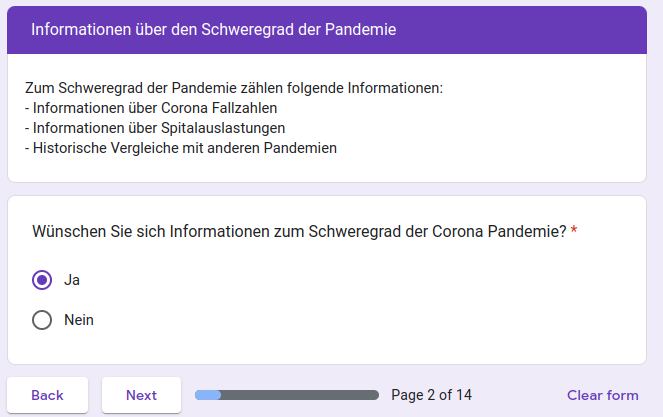
\includegraphics[width=12cm]{images/online_formular_sections.png}
    \centering
    \caption{Modularer Aufbau des Fragebogens (Eigene Darstellung)}
    \label{fig:online_formular_sections}
\end{figure}

\clearpage
Haben die Probanden Ihr Interesse für eine bestimmte Kategorie geäussert, wurden Sie genauer dazu befragt. Hierzu mussten Sie mithilfe einer 5-stufigen Likert Scala angeben wie interessiert sie an den jeweiligen Subkategorien sind (siehe Abbildung \ref{fig:online_formular_identification_of_relevant_information}).

\begin{figure}[h]
    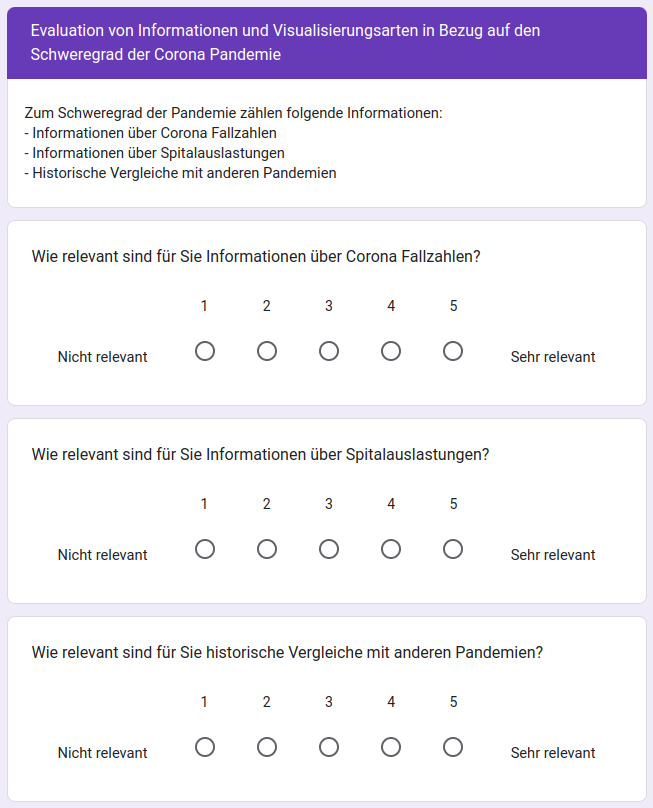
\includegraphics[width=12cm]{images/online_formular_identification_of_relevant_information.png}
    \centering
    \caption{Identifizierung der relevanten Informationen (Eigene Darstellung)}
    \label{fig:online_formular_identification_of_relevant_information}
\end{figure}

\clearpage
Anschliessend wurden aufgrund der definierten Anwendungsfälle sowie den identifizierten Datenvisualisierungen (siehe Kapitel \ref{ch:analysis_of_codebook} sowie \ref{ch:identification_of_use_cases}) die Probanden befragt, welchen Typ von Datenvisualisierung Sie für den Anwendungsfall verwenden würden. Hierbei wurde ebenfalls die Möglichkeit zur Verfügung gestellt eine andere Datenvisualisierung mithilfe der ``Other`` Option auszuwählen (siehe Abbildung \ref{fig:online_formular_use_cases_and_visualizations})

\begin{figure}[h]
    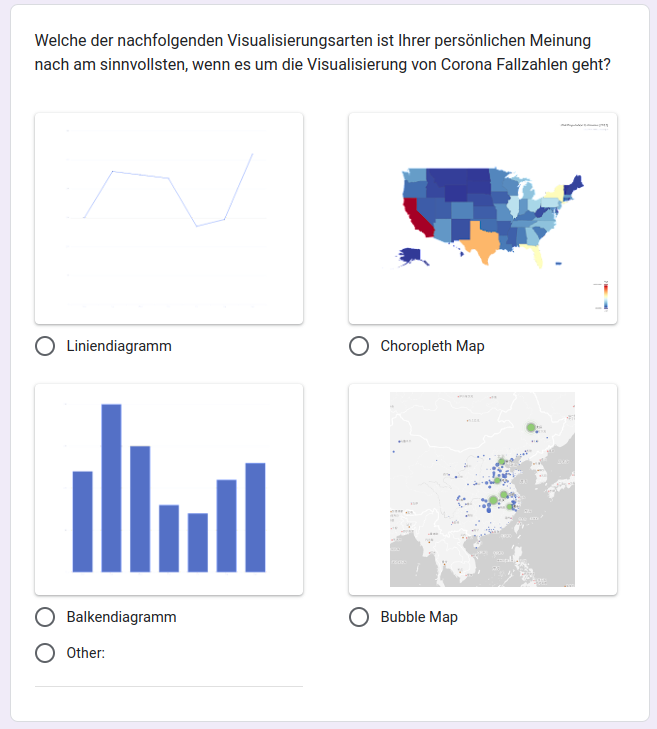
\includegraphics[width=10cm]{images/online_formular_use_cases_and_visualizations.png}
    \centering
    \caption{Identifizierung von Datenvisualisierungen pro Anwendungsfall (Eigene Darstellung)}
    \label{fig:online_formular_use_cases_and_visualizations}
\end{figure}

Dieses Vorgehen wurde für sämtliche Anwendungsfälle pro Subkategorie wiederholt. Ein Spezialfall bildete hierbei Subkategorie ``Erklärungen zum Coronavirus im Allgemeinen``. Hier wurden den Probanden explizit keine Vorschläge für Datenvisualisierungen unterbeitet sondern nur ein Eingabefeld zur Verfügung gestellt (siehe Abbildung \ref{fig:online_formular_special_case_for_general_information}).

\begin{figure}[h]
    
\includegraphics[width=10cm]{images/online_formular_special_case_for_general_information.png}
    \centering
    \caption{Identifizierung von Datenvisualisierungen zur Erklärung von Allgemeinen Informationen in Bezug auf Corona (Eigene Darstellung)}
    \label{fig:online_formular_special_case_for_general_information}
\end{figure}

\clearpage
Am Schluss des Fragebogens ist noch der Informationsbedarf in Bezug auf die Schweiz oder die gesamte Welt ermittelt worden (siehe Abbildung \ref{fig:online_formular_worldwide_switzerland_information_need}).

\begin{figure}[h]
    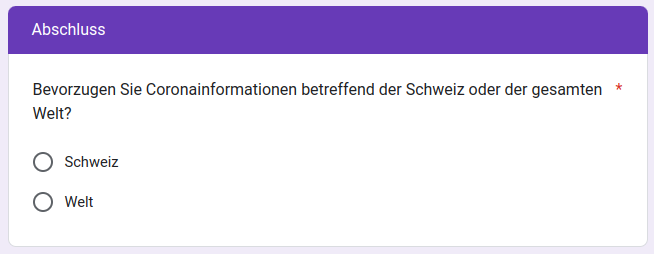
\includegraphics[width=10cm]{images/online_formular_worldwide_switzerland_information_need.png}
    \centering
    \caption{Ermittlung des Informationsbedarfs in Bezug auf die Schweiz oder die Welt (Eigene Darstellung)}
    \label{fig:online_formular_worldwide_switzerland_information_need}
\end{figure}

Zusätzlich wurde noch der Informationsbedarf pro Kategorie mithilfe einer 5-stufigen Likert Skala evaluiert worden (siehe Abbildung \ref{fig:online_formular_likert_scale_category}).

\begin{figure}[h]
    
\includegraphics[width=10cm]{images/online_formular_likert_scale_category.png}
    \centering
    \caption{Ermittlung des Informationsbedarfs pro Kategorie (Eigene Darstellung)}
    \label{fig:online_formular_likert_scale_category}
\end{figure}

Der Abschluss des Fragebogens bildete die Frage, ob der Proband bereits Erfahrungen mit Dashboards in Bezug auf Corona gemacht hat, was zugleich auch als Brückenschlag für das nachfolgende Interview diente (siehe Abbildung \ref{fig:online_formular_experience_with_dashboards}).

\begin{figure}[h]
    
\includegraphics[width=10cm]{images/online_formular_experience_with_dashboards.png}
    \centering
    \caption{Ermittlung der Erfahrung von Dashboards (Eigene Darstellung)}
    \label{fig:online_formular_experience_with_dashboards}
\end{figure}

\subsubsection{Interview}
Als Grundlage für das Interview diente der erstellte Interviewleitfaden (siehe Kapitel \ref{ch:creation_of_interview_guide}). Mithilfe des think-aloud Ansatzes und der Screen Sharing Funktionalität von Google Meets war es möglich bei Unklarheiten direkt nachzufragen und so an wertvolles Nutzerfeedback zu gelangen. Während des Interviews wurde das Feedback stichwortartig festgehalten.

\subsection{Auswertung des Untersuchungsinstrumentes}
Nachfolgend werden die wichtigsten Ergebnisse in Bezug auf den Online Fragebogen sowie das Interview thematisiert und entsprechende Anforderungen an ein Artefakt abgeleitet. Da es sich bei den Interviews nicht um Experteninterviews handelt, wurde auf eine Transkription verzichtet.

\subsubsection{Online Fragebogen}
Durch die Verwendung von Google Forms war eine automatische Auswertung der Ergebnisse möglich. Nachfolgend wird auf die wichtigsten Punkte eingegangen.\\

\noindent
\textbf{Informationsbedarf betreffend den Kategorien}
\newline
\indent
Insgesamt besteht bei allen Probanden ein Interesse an sämtlichen Kategorien. Lediglich ein Proband gab an, dass kein Interesse an den Kategorien ``Informationen über den Einfluss der Pandemie`` sowie ``Informationen zur Risikoverminderung des Corona Virus`` zu haben (siehe Abbildung \ref{fig:online_formular_evaluation_impact_of_covid} und \ref{fig:online_formular_evaluation_risk_mitigation}).


\begin{figure}[h]
    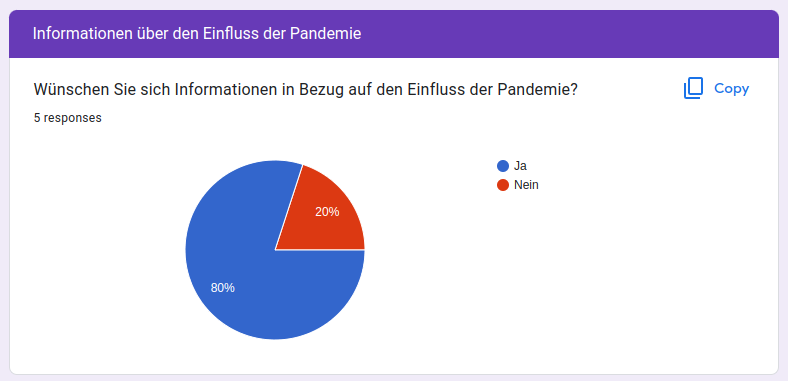
\includegraphics[width=10cm]{images/online_formular_evaluation_impact_of_covid.png}
    \centering
    \caption{Interessensbekundung in der Kategorie ``Informationen über den Einfluss der Pandemie`` (Eigene Darstellung)}
    \label{fig:online_formular_evaluation_impact_of_covid}
\end{figure}

\begin{figure}[h]
    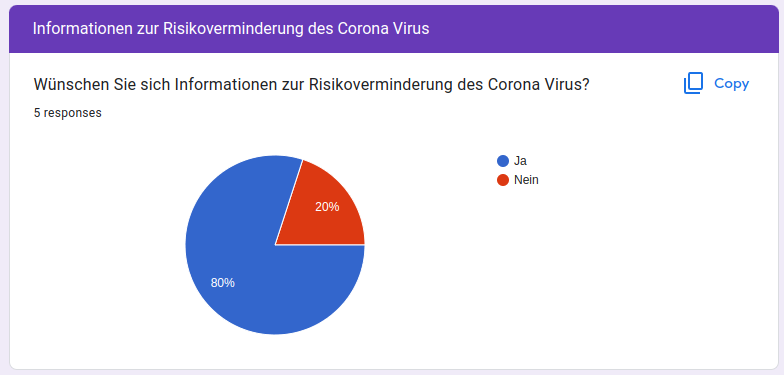
\includegraphics[width=10cm]{images/online_formular_evaluation_risk_mitigation.png}
    \centering
    \caption{Interessensbekundung in der Kategorie ``Informationen zur Risikoverminderung des Corona Virus`` (Eigene Darstellung)}
    \label{fig:online_formular_evaluation_risk_mitigation}
\end{figure}

\clearpage
Aufgrund der eingeführten Linkert Skalen war zudem eine Mittelwertberechnung des Interessenswertes pro  Kategorie möglich. Tabelle \ref{table:interest_per_category} zeigt die berechneten Mittelwerte pro Kategorie auf. Bei den Spaltenüberschriften gilt ein Wert von 1 als nicht relevant und ein Wert von 5 als sehr relevant. In den Zeilen stehen jeweils die Anzahl der Probanden. Durch ermittlung des Durchschnittswertes wird ersichtlich dass die Kategorien ``Informationen zum Schweregrad der Pandemie`` sowie ``Informationen zur Risikoverminderung des Corona Virus`` als wichtigste Kategorien wahrgenommen werden.

% Begin Table relevance of categories
\begin{table}[h]
\centering
\resizebox{\textwidth}{!}{%
\begin{tabular}{@{}lllllll@{}}
\toprule
\textbf{Kategorie} & \textbf{1} & \textbf{2} & \textbf{3} & \textbf{4} & \textbf{5} & \textbf{Durchschnittswert} \\ \midrule
Informationen zum Schweregrad der Pandemie & 0 & 0 & 0 & 2 & 3 & \textbf{4.6} \\ \midrule
Informationen zu Trendvorhersagen & 0 & 0 & 1 & 3 & 1 & 4 \\ \midrule
Informationen zum Einfluss der Pandemie & 1 & 1 & 2 & 1 & 0 & 2.6 \\ \midrule
Informationen zur Erklärung der Natur des Corona Virus & 0 & 0 & 2 & 1 & 2 & 4 \\ \midrule
Informationen zur Risikoverminderung des Corona Virus & 0 & 0 & 1 & 2 & 2 & \textbf{4.2} \\ \midrule
Informationen über Verletzlichkeit bestimmter Personengruppen & 0 & 0 & 2 & 2 & 1 & 3.8 \\ \bottomrule
\end{tabular}%
}
\caption{Interessenzrelevanz der Probanden pro Kategorie (Eigene Darstellung)}
\label{table:interest_per_category}
\end{table}
% End Table relevance of categories


\noindent
\textbf{Informationsbedarf betreffend den Subkategorien}
\newline
\indent
Für die Subkategorien sind ebenfalls die Durchschnittswerte aufgrund der Linkert Skala ermittelt worden. Zusätzlich wurden die am häufigsten verwendeten Datenvisualisierung pro Anwendungsfall ermittelt. Für jede Subkategorie sind ebenfalls die wichtigsten Bemerkungen der Probanden aufgeführt.\\

\noindent
\textit{Schweregrad der Pandemie}
\newline
\indent
In Bezug auf die Subkategorien für den Schweregrad der Pandemien sind die Corona Fallzahlen sowie die Spitalaulastungen als am Wichtigsten erachtet worden (siehe Tabelle \ref{table:interest_subcategory_severity_of_pandemic}).

% Begin Table information need for subcategory Severity of Pandemic
\begin{table}[h]
\centering
\resizebox{\textwidth}{!}{%
\begin{tabular}{@{}lllllll@{}}
\toprule
\textbf{Kategorie} & \textbf{1} & \textbf{2} & \textbf{3} & \textbf{4} & \textbf{5} & \textbf{Durchschnittswert} \\ \midrule
Informationen zu Corona Fallzahlen & 0 & 0 & 0 & 3 & 2 & \textbf{4.4} \\ \midrule
Informationen zu Spitalauslastungen & 0 & 0 & 1 & 1 & 3 & \textbf{4.4} \\ \midrule
Historische Vergleiche mit anderen Pandemien & 0 & 1 & 2 & 2 & 0 & 3.2 \\ \bottomrule
\end{tabular}%
}
\caption{Interessenzrelevanz der Probanden für Unterkategorien des Bereichs ``Schweregrad der Pandemie`` (Eigene Darstellung)}
\label{table:interest_subcategory_severity_of_pandemic}
\end{table}
% End Table information need for subcategory Severity of Pandemic

\clearpage
Als wichtigste Datenvisualisierungen in Bezug auf die definierten Anwendungsfälle sind Linien sowie Balkendiagramme identifiziert worden (siehe Tabelle \ref{table:data_visualizations_severity_of_pandemic}). Nebst diesen Datenvisualisierungen ist gemäss Aussagen der Probanden zudem eine rein textuelle Darstellung mithilfe von absoluten Zahlen erwünscht.

% Start Table data visualizations for subcategory Severity of Pandemic
\begin{table}[h]
\centering
\resizebox{\textwidth}{!} & 20\% & 20\% & 20\% & 0\% \\ \midrule
Visualisierung von Spitalauslastungen & \textbf{40\%} & 0\% & \textbf{40\%} & 20\% & 0\% \\ \midrule
Historische Vergleiche mit anderen Pandemien auf Fallzahlen & \textbf{40\%} & 0\% & \textbf{40\%} & 0\% & 20\% \\ \bottomrule
\end{tabular}%
}
\caption{Ausgewählte Datenvisualisierungen pro Anwendungsfälle für den Bereich ``Schweregrad der Pandemie`` (Eigene Darstellung)}
\label{table:data_visualizations_severity_of_pandemic}
\end{table}
% End Table data visualizations for subcategory Severity of Pandemic

\noindent
\textit{Trendvorhersagen zur Pandemie}
\newline
\indent
Sowohl Vorhersagen zu Todesfälle als auch zu Ansteckungszahlen sind den Probanden gleichermassen wichtig (siehe Tabelle \ref{table:interest_subcategory_forecast}).

% Begin Table information need for category forecasting
\begin{table}[h]
\centering
\resizebox{\textwidth}{!}{%
\begin{tabular}{@{}lllllll@{}}
\toprule
\textbf{Kategorie} & \textbf{1} & \textbf{2} & \textbf{3} & \textbf{4} & \textbf{5} & \textbf{Durchschnittswert} \\ \midrule
Trendvorhersage zu Ansteckungszahlen & 0 & 0 & 2 & 2 & 1 & \textbf{3.8} \\ \midrule
Trendvorhersagen zu Todesfällen & 0 & 1 & 0 & 3 & 1 & \textbf{3.8} \\ \bottomrule
\end{tabular}%
}
\caption{Interessenzrelevanz der Probanden für Unterkategorien des Bereichs ``Trendvorhersagen zur Pandemie`` (Eigene Darstellung)}
\label{table:interest_subcategory_forecast}
\end{table}
% End Table information need for category forecasting

Das Liniendiagramm wurde hierbei als bevorzugte Datenvisualisierung von den Probanden gewählt (siehe Tabelle \ref{table:data_visualizations_forecast_of_pandemic}).

% Start Table Data Visualizations for forecasting
\begin{table}[h]
\centering
\resizebox{\textwidth}{!} & 0\% & 20\% & 0\% \\ \midrule
Visualisierung von Corona Todesfällen & \textbf{60\%} & 0\% & 20\% & 20\% \\ \bottomrule
\end{tabular}%
}
\caption{Ausgewählte Datenvisualisierungen pro Anwendungsfall für den Bereich ``Trendvorhersagen zur Pandemie`` (Eigene Darstellung)}
\label{table:data_visualizations_forecast_of_pandemic}
\end{table}
% End Table Data Visualizations for forecasting

\clearpage
\noindent
\textit{Einfluss der Pandemie}
\newline
\indent
Vier von fünf befragten Probanden haben sich für den Einfluss der Pandemie interessiert (siehe Abbildung \ref{fig:online_formular_evaluation_impact_of_covid}). Hierbei hat sich der Einfluss auf den Bereich Ökonomie sowie der Einfluss von rechtlichen Vorschriften (beispielsweise Corona Lockdown) als relevant erwiesen (siehe Tabelle \ref{table:interest_subcategory_influence}).

\begin{table}[h]
\centering
\resizebox{\textwidth}{!}{%
\begin{tabular}{@{}lllllll@{}}
\toprule
\textbf{Kategorie} & \textbf{1} & \textbf{2} & \textbf{3} & \textbf{4} & \textbf{5} & \textbf{Durchschnittswert} \\ \midrule
Einfluss auf Ökonomie & 0 & 0 & 1 & 1 & 2 & \textbf{4.25} \\ \midrule
Einfluss auf Soziales Gefüge & 0 & 0 & 2 & 2 & 0 & 3.5 \\ \midrule
Einfluss auf Umwelt & 0 & 0 & 2 & 1 & 1 & 3.75 \\ \midrule
Einfluss auf Politik & 0 & 1 & 2 & 0 & 1 & 3.25 \\ \midrule
Einfluss einer rechtlichen Vorschrift & 0 & 0 & 0 & 1 & 3 & \textbf{4.75} \\ \bottomrule
\end{tabular}%
}
\caption{Interessenzrelevanz der Probanden für Unterkategorien des Bereichs ``Einfluss der Pandemie`` (Eigene Darstellung)}
\label{table:interest_subcategory_influence}
\end{table}

Die präferierten Datenvisualisierungen sind in diesem Bereich nicht eindeutig zu identifizieren. Dies kann unter anderem am breiten Spektrum der Themengebiete liegen. Jedoch haben die Probanden besonders in Bezug auf den Luftverkehr ein grosses Interesse an Heat Maps geäussert (siehe Tabelle \ref{table:data_visualizations_impact_of_pandemic}).

\begin{table}[h]
\centering
\resizebox{\textwidth}{!}{%
\begin{tabular}{@{}lllllllll@{}}
\toprule
\textbf{Anwendungsfall} & \textbf{Liniendiagramm} & \textbf{Choropleth Map} & \textbf{Balkendiagramm} & \textbf{Gestapeltes Balkendiagramm} & \textbf{Kuchendiagramm} & \textbf{Scatter Plot} & \textbf{Heat Map} & \textbf{Bubble Map} \\ \midrule
\begin{tabular}[c]{@{}l@{}}Einfluss von Corona auf Umsatzzahlen\\ der IT Branche\end{tabular} & 25\% & 0\% & \textbf{50\%} & 25\% & 0\% & 0\% & 0\% & 0\% \\ \midrule
Anzahl Personen welche soziale Unterstützung beziehen & 0\% & 0\% & \textbf{50\%} & 20\% & 25\% & 25\% & 0\% & 0\% \\ \midrule
Anzahl Flüge im Luftverkehr & 0\% & 0\% & 25\% & 0\% & 0\% & 0\% & \textbf{75\%} & 0\% \\ \midrule
Anzahl Abstimmungen zu einem Corona Thema & 25\% & \textbf{50\%} & 0\% & 0\% & 0\% & 0\% & 0\% & 25\% \\ \midrule
Einfluss des Corona Lockdowns auf Fallzahlen & \textbf{75\%} & 0\% & 25\% & 0\% & 0\% & 0\% & 0\% & 0\% \\ \bottomrule
\end{tabular}%
}
\caption{Ausgewählte Datenvisualisierungen pro Anwendungsfall für den Bereich ``Einfluss der Pandemie`` (Eigene Darstellung)}
\label{table:data_visualizations_impact_of_pandemic}
\end{table}

\clearpage
\noindent
\textit{Erklärung der Natur}
\newline
\indent
Informationen in Bezug auf Symptome, Diagnosen sowie Behandlungen scheinen den Probanden wichtig zu sein. Dies gilt ebenfalls für Informationen in Bezug auf die Übertragung des Virus (siehe Tabelle \ref{table:interest_subcategory_nature_of_pandemic}).  Als weniger relevant gaben die Probanden Informationen zu Contact Tracing an. Hauptgrund hierfür war gemäss den Probanden dass die Covid App nicht zufriedenstellend war.

\begin{table}[h]
\centering
\resizebox{\textwidth}{!}{%
\begin{tabular}{@{}lllllll@{}}
\toprule
\textbf{Kategorie} & \textbf{1} & \textbf{2} & \textbf{3} & \textbf{4} & \textbf{5} & \textbf{Durchschnittswert} \\ \midrule
Information zum Virus im Allgemeinen & 0 & 0 & 3 & 2 & 0 & 3.4 \\ \midrule
Informationen zu Symptomen, Diagnosen und Behandlungen & 0 & 0 & 1 & 3 & 1 & \textbf{4} \\ \midrule
Informationen zur Übertragung des Virus & 0 & 0 & 1 & 3 & 1 & \textbf{4} \\ \midrule
Informationen zu Contact Tracing & 1 & 1 & 2 & 0 & 1 & 2.8 \\ \bottomrule
\end{tabular}%
}
\caption{Interessenzrelevanz der Probanden für Unterkategorien des Bereichs ``Erklärung der Natur`` (Eigene Darstellung)}
\label{table:interest_subcategory_nature_of_pandemic}
\end{table}

In Bezug auf die Datenvisualisierungen wurde zur Visualisierungen von Allgemeinen Informationen zum Coronavirus ein \gls{faq} Bereich gewünscht (siehe Abbildung \ref{fig:online_formular_visualization_for_general_covid_information}).

 \begin{figure}[h]
    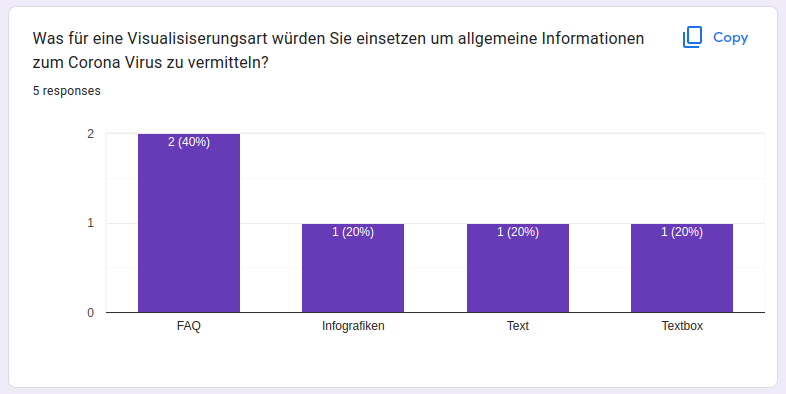
\includegraphics[width=14cm]{images/online_formular_visualization_for_general_covid_information.png}
    \centering
    \caption{Datenvisualisierung für allgemeine Informationen zu Corona (Eigene Darstellung)}
    \label{fig:online_formular_visualization_for_general_covid_information}
\end{figure}

\clearpage
In Bezug auf die umgesetzten Schutzmassnahmen ist kein Favorit der Probanden erkennbar. Sowohl beim Anwendungsfall bezüglich der Verbreitung als auch bei den eingereichten Covid Codes via SwissCovid empfinden die Probanden das Balkendiagramm als passende Option. Nebst dem Balkendiagramm wurde von Probanden die Darstellung als reiner Text mit einfachem Zahlenwert gewünscht (siehe Tabelle \ref{table:data_visualizations_explain_nature}).

\begin{table}[h]
\centering
\resizebox{\textwidth}{!}{%
\begin{tabular}{@{}llllllll@{}}
\toprule
\textbf{Anwendungsfall} & \textbf{Liniendiagramm} & \textbf{Choropleth Map} & \textbf{Balkendiagramm} & \textbf{Bubble Map} & \textbf{Kuchendiagramm} & \textbf{Darstellung als Text} & \textbf{Kein Interesse} \\ \midrule
\begin{tabular}[c]{@{}l@{}}Aufzeigen wie viel Prozent der Bevölkerung\\ Schutzmassnahmen bereits umsetzen\end{tabular} & 20\% & 20\% & 20\% & 20\% & 20\% & 0\% & 20\% \\ \midrule
\begin{tabular}[c]{@{}l@{}}Verbreitung des Corona Virus über Hände\\ schütteln etc.\end{tabular} & 0\% & 0\% & \textbf{100\%} & 0\% & 0\% & 0\% & 0\% \\ \midrule
\begin{tabular}[c]{@{}l@{}}Anahl eingereichter Covid Codes\\ über SwissCovid\end{tabular} & 20\% & 0\% & \textbf{40\%} & 0\% & 0\% & \textbf{40\%} & 0\% \\ \bottomrule
\end{tabular}%
}
\caption{Ausgewählte Datenvisualisierungen pro Anwendungsfall für den Bereich ``Erklärung der Natur`` (Eigene Darstellung)}
\label{table:data_visualizations_explain_nature}
\end{table}

\noindent
\textit{Informationen zur Risikoverminderung}
\newline
\indent
Informationenin betreffend Hygiene sowie Massnahmen um die Corona Kurve flach zu halten sind die präferierten Kategorien der Probanden (siehe Tabelle \ref{table:interest_subcategory_risk_mitigation}). Eine Person der 5 befragten Probanden hat sich hierbei dazu entschlossen keine Meinung zu diesem Themenbereich abzugeben (siehe Abbildung \ref{fig:online_formular_evaluation_risk_mitigation}). 

\begin{table}[h]
\centering
\resizebox{\textwidth}{!}{%
\begin{tabular}{@{}lllllll@{}}
\toprule
\textbf{Kategorie} & \textbf{1} & \textbf{2} & \textbf{3} & \textbf{4} & \textbf{5} & \textbf{Durchschnittswert} \\ \midrule
Informationen zu Social Distancing & 0 & 1 & 1 & 2 & 0 & 3.25 \\ \midrule
Informationen zu Schutzequipment & 0 & 1 & 1 & 2 & 0 & 3.25 \\ \midrule
Informationen zu Hygiene & 0 & 0 & 1 & 1 & 2 & \textbf{4.25} \\ \midrule
Flatten the Curve & 0 & 0 & 2 & 2 & 0 & \textbf{3.5} \\ \bottomrule
\end{tabular}%
}
\caption{Interessenzrelevanz der Probanden für Unterkategorien des Bereichs ``Informationen zur Risikoverminderung`` (Eigene Darstellung)}
\label{table:interest_subcategory_risk_mitigation}
\end{table}

Als favorisierte Datenvisualisierungen sind auch hier Balken sowie Liniendiagramme von Relevanz. Jedoch haben die Probanden in Bezug auf die Wirksamkeit der Schutzmasken ebenfalls das Radar Chart angesprochen, mithilfe dessen die Wirksamkeit einer Maske in verschiedenen Ausprägungen (Schutz gegen Partikel etc.) visualisiert werden kann (siehe Tabelle \ref{table:data_visualizations_risk_mitigation}).

\begin{table}[h]
\centering
\resizebox{\textwidth}{!} & \textbf{50\%} & 0\% & 0\% & 0\% & 0\% & 0\% \\ \midrule
Wirksamkeit einer Schutzmaske aufzeigen & 0\% & 0\% & 25\% & 0\% & \textbf{75\%} & 0\% & 0\% \\ \midrule
\begin{tabular}[c]{@{}l@{}}Wirksamkeit von Hygienemassnahmen auf\\ Corona Fallzahlen\end{tabular} & 0\% & \textbf{50\%} & 0\% & 0\% & \textbf{50\%} & 0\% & 0\% \\ \bottomrule
\end{tabular}%
}
\caption{Ausgewählte Datenvisualisierungen pro Anwendungsfall für den Bereich ``Informationen zur Risikoverminderung`` (Eigene Darstellung)}
\label{table:data_visualizations_risk_mitigation}
\end{table}

\clearpage
\noindent
\textit{Verletzlichkeit von Personengruppen}
\newline
\indent
Informationen betreffend der Personen einer bestimmten Altersgruppe wurde als relevant erachtet. Nationalität sowie Geschlecht sind gemäss den Probanden weniger wichtig (siehe Tabelle \ref{table:interest_subcategory_vulnerability}).

\begin{table}[h]
\centering
\resizebox{\textwidth}{!}{%
\begin{tabular}{@{}lllllll@{}}
\toprule
\textbf{Kategorie} & \textbf{1} & \textbf{2} & \textbf{3} & \textbf{4} & \textbf{5} & \textbf{Durchschnittswert} \\ \midrule
Informationen zu Personen einer bestimmten Altersgruppe & 0 & 0 & 0 & 2 & 3 & \textbf{4.6} \\ \midrule
Informationen zu Personen eines bestimmten Geschlechts & 0 & 2 & 2 & 1 & 0 & 2.8 \\ \midrule
Informationen zu Personen einer bestimmten Nationalität & 2 & 1 & 1 & 1 & 0 & 2.2 \\ \bottomrule
\end{tabular}%
}
\caption{Interessenzrelevanz der Probanden für Unterkategorien des Bereichs ``Verletzlichkeit von Personengruppen`` (Eigene Darstellung)}
\label{table:interest_subcategory_vulnerability}
\end{table}

Als bevorzugte Visualisierungsart wurde primär das Balkendiagramm gewählt (siehe Tabelle \ref{table:data_visualizations_vulnerability}).

\begin{table}[h]
\centering
\resizebox{\textwidth}{!}{%
\begin{tabular}{@{}lllllll@{}}
\toprule
\textbf{Anwendungsfall} & \textbf{Liniendiagramm} & \textbf{Balkendiagramm} & \textbf{Bubble Map} & \textbf{Choropleth Map} & \textbf{Kuchendiagramm} & \textbf{Nicht relevant} \\ \midrule
Informationen zu Personen einer bestimmten Altersgruppe & 0\% & \textbf{100\%} & 0\% & 0\% & 0\% & 0\% \\ \midrule
Informationen zu Personen eines bestimmten Geschlechts & 0\% & \textbf{60\%} & 20\% & 0\% & 20\% & 0\% \\ \midrule
Informationen zu Personen einer bestimmten Nationalität & 0\% & \textbf{60\%} & 0\% & 20\% & 0\% & 20\% \\ \bottomrule
\end{tabular}%
}
\caption{Ausgewählte Datenvisualisierungen pro Anwendungsfall für den Bereich ``Verletzlichkeit von Personengruppen`` (Eigene Darstellung)}
\label{table:data_visualizations_vulnerability}
\end{table}


\noindent
\textbf{Konsumverhalten von Corona Informationen}
\newline
\indent
Bezüglich des Informationsbedarfs bevorzugen rund 80\% der befragten Probanden Informationen über die ganze Welt. Lediglich eine Person gab an nur an Informationen zur Schweiz interessiert zu sein (siehe Abbildung \ref{fig:information_need_worldwide_switzerland}).

\begin{figure}[h]
    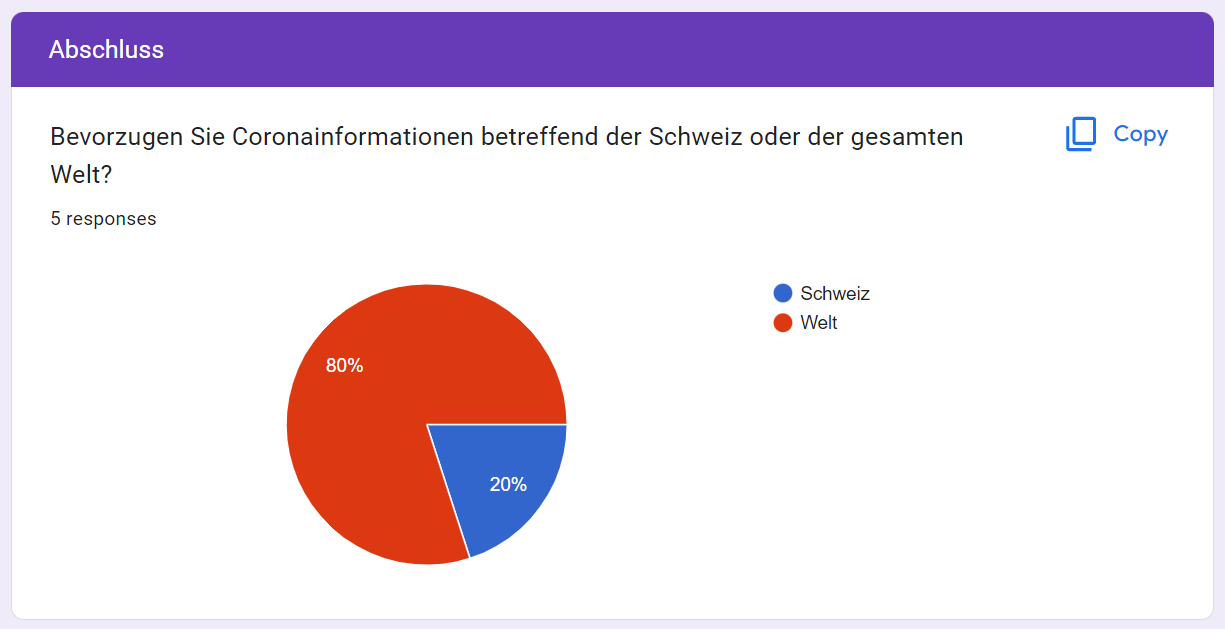
\includegraphics[width=14cm]{images/information_need_worldwide_switzerland.png}
    \centering
    \caption{Informationsbedarf Vergleich weltweit - Schweiz (Eigene Darstellung)}
    \label{fig:information_need_worldwide_switzerland}
\end{figure}

\clearpage
In Bezug auf die konsumierten Medien ist das Internet die primäre Informationsquelle der Millennials (siehe Tabelle \ref{table:information_consumption_medium}). Die Probanden gaben zudem an, dass Sie sich auch über das Radio sowie Online Zeitungen zum Thema Corona informierten.

\begin{table}[h]
\centering
\resizebox{\textwidth}{!}{%
\begin{tabular}{@{}lllllll@{}}
\toprule
\textbf{Informationsmedium} & \textbf{1} & \textbf{2} & \textbf{3} & \textbf{4} & \textbf{5} & \textbf{Durchschnittswert} \\ \midrule
Internet & 0 & 0 & 3 & 2 & 0 & \textbf{3.4} \\ \midrule
Soziale Medien & 1 & 3 & 0 & 0 & 1 & 2.4 \\ \midrule
Printmedien & 2 & 1 & 2 & 0 & 0 & 2 \\ \bottomrule
\end{tabular}%
}
\caption{Bevorzugte Medien der Millennials für den Informationskonsum in Bezug auf Corona (Eigene Darstellung)}
\label{table:information_consumption_medium}
\end{table}

\subsubsection{Interview}
60\% der befragten Probanden gaben an bereits Erfahrungen mit einem Dashboard gemacht zu haben. Nachfolgend wird auf die wichtigsten Aussagen der Probanden zu den einzelnen Teilbereichen des erstellten Interviewleitfadens (siehe Kapitel \ref{ch:creation_of_interview_guide}) eingegangen. Die hier aufgeführten Ergebnisse basieren auf einem erstellten Mindmap auf Basis der Gesprächsnotizen. Das Mindmap kann dem Anhang \ref{app:interview_mind_map} entnommen werden.\\

\clearpage
\noindent
\textbf{Positive Aspekte}
\newline
\indent
Beim Besuch des Corona Dashboards der Schweiz (siehe Abbildung \ref{fig:corona_dashboard_switzerland}) haben die Probanden das Design des Dashboards aufgrund der korrekten Farbwahl (Pastelfarben) sowie der ansprechenden Typografie als angenehm empfunden. Auch wurde die Aufteilung in spezifische Bereiche mit Hilfe von Tabs als hilfreich wahrgenommen. In Bezug auf die Visualisierungen ist das Hervorheben von wichtigen Informationen mit entsprechenden Farben (siehe Kapitel \ref{ch:introduction_colors}) als positiv erachtet worden. Auch ist die Auswahl der Datenvisualisierungen nicht zu breit gestreut und einfach gehalten, was den Probanden ebenfalls als positiven Aspekt aufgefallen ist. 

\begin{figure}[h]
    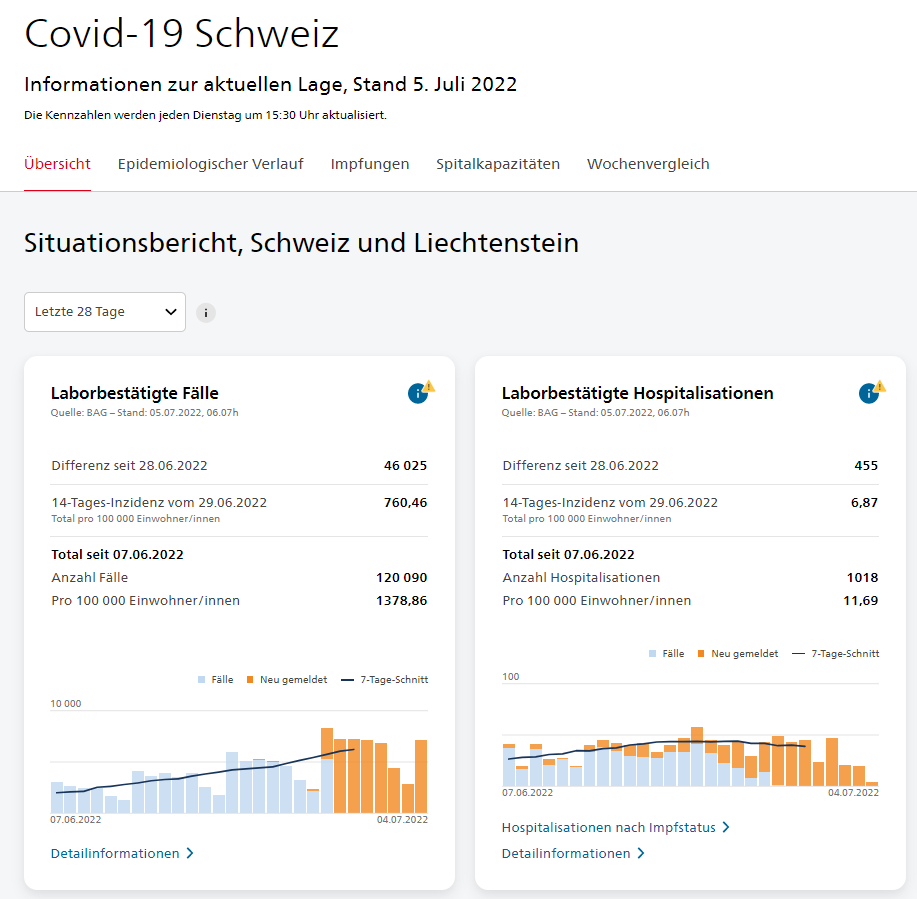
\includegraphics[width=14cm]{images/covid_dashboard_switzerland.png}
    \centering
    \caption{Corona Virus Dashboard der Schweiz ~\citep{corona_dashboard_switzerland}}
    \label{fig:corona_dashboard_switzerland}
\end{figure}

\noindent
\textbf{Negative Aspekte}
\newline
\indent
Als weniger positiv haben die Probanden die Menge an Informationen aufgeführt. Gemäss Aussagen der Probanden musste zudem viel geklickt werden um die passende Information zu finden.

\clearpage
\noindent
\textbf{Wünschenswerte Aspekte}
\newline
\indent
Ein wünschenswerter Aspekt möchten die Probanden gerne die Möglichkeit haben, die Datenvisualisierungen ``on the fly`` zu wechseln. Zudem sollte es Freude mit den Grafiken zu interagieren.\\

\noindent
\textbf{Filterfunktionalitäten}
\newline
\indent
Filterfunktionalitäten sind den Millennials sehr wichtig und werden als zentrale Grundvoraussetzung für ein Dashboard angesehen. Als relevanteste Filter wurden Regions sowie Zeitfilter genannt. Zudem soll der Filter beim Scrollen durch die Webseite ```mitfliessen``. Wünschenswert wäre ebenfalls die Möglichkeit aus einer Liste von Filtern auswählen zu können.\\

\noindent
\textbf{Datenvisualisierungen}
\newline
\indent
Als eindrucksvolle Datenvisualisierung wurde die Gebietsstufenkarte (Choropleth Map) genannt. Hier hat den Probanden besonders die Interaktivität und die einfache Verständlichkeit gefallen (siehe Abbildung \ref{fig:covid_dashboard_switzerland_choropleth_map}). Nebst der Gebietsstufenkarte sind auch Heatmaps sowie Visualisierungen welche den epidemiologischen Verlauf von laborbestätigten Fällen und Hospitalisationen aufzeigt von Interesse.

\begin{figure}[h]
    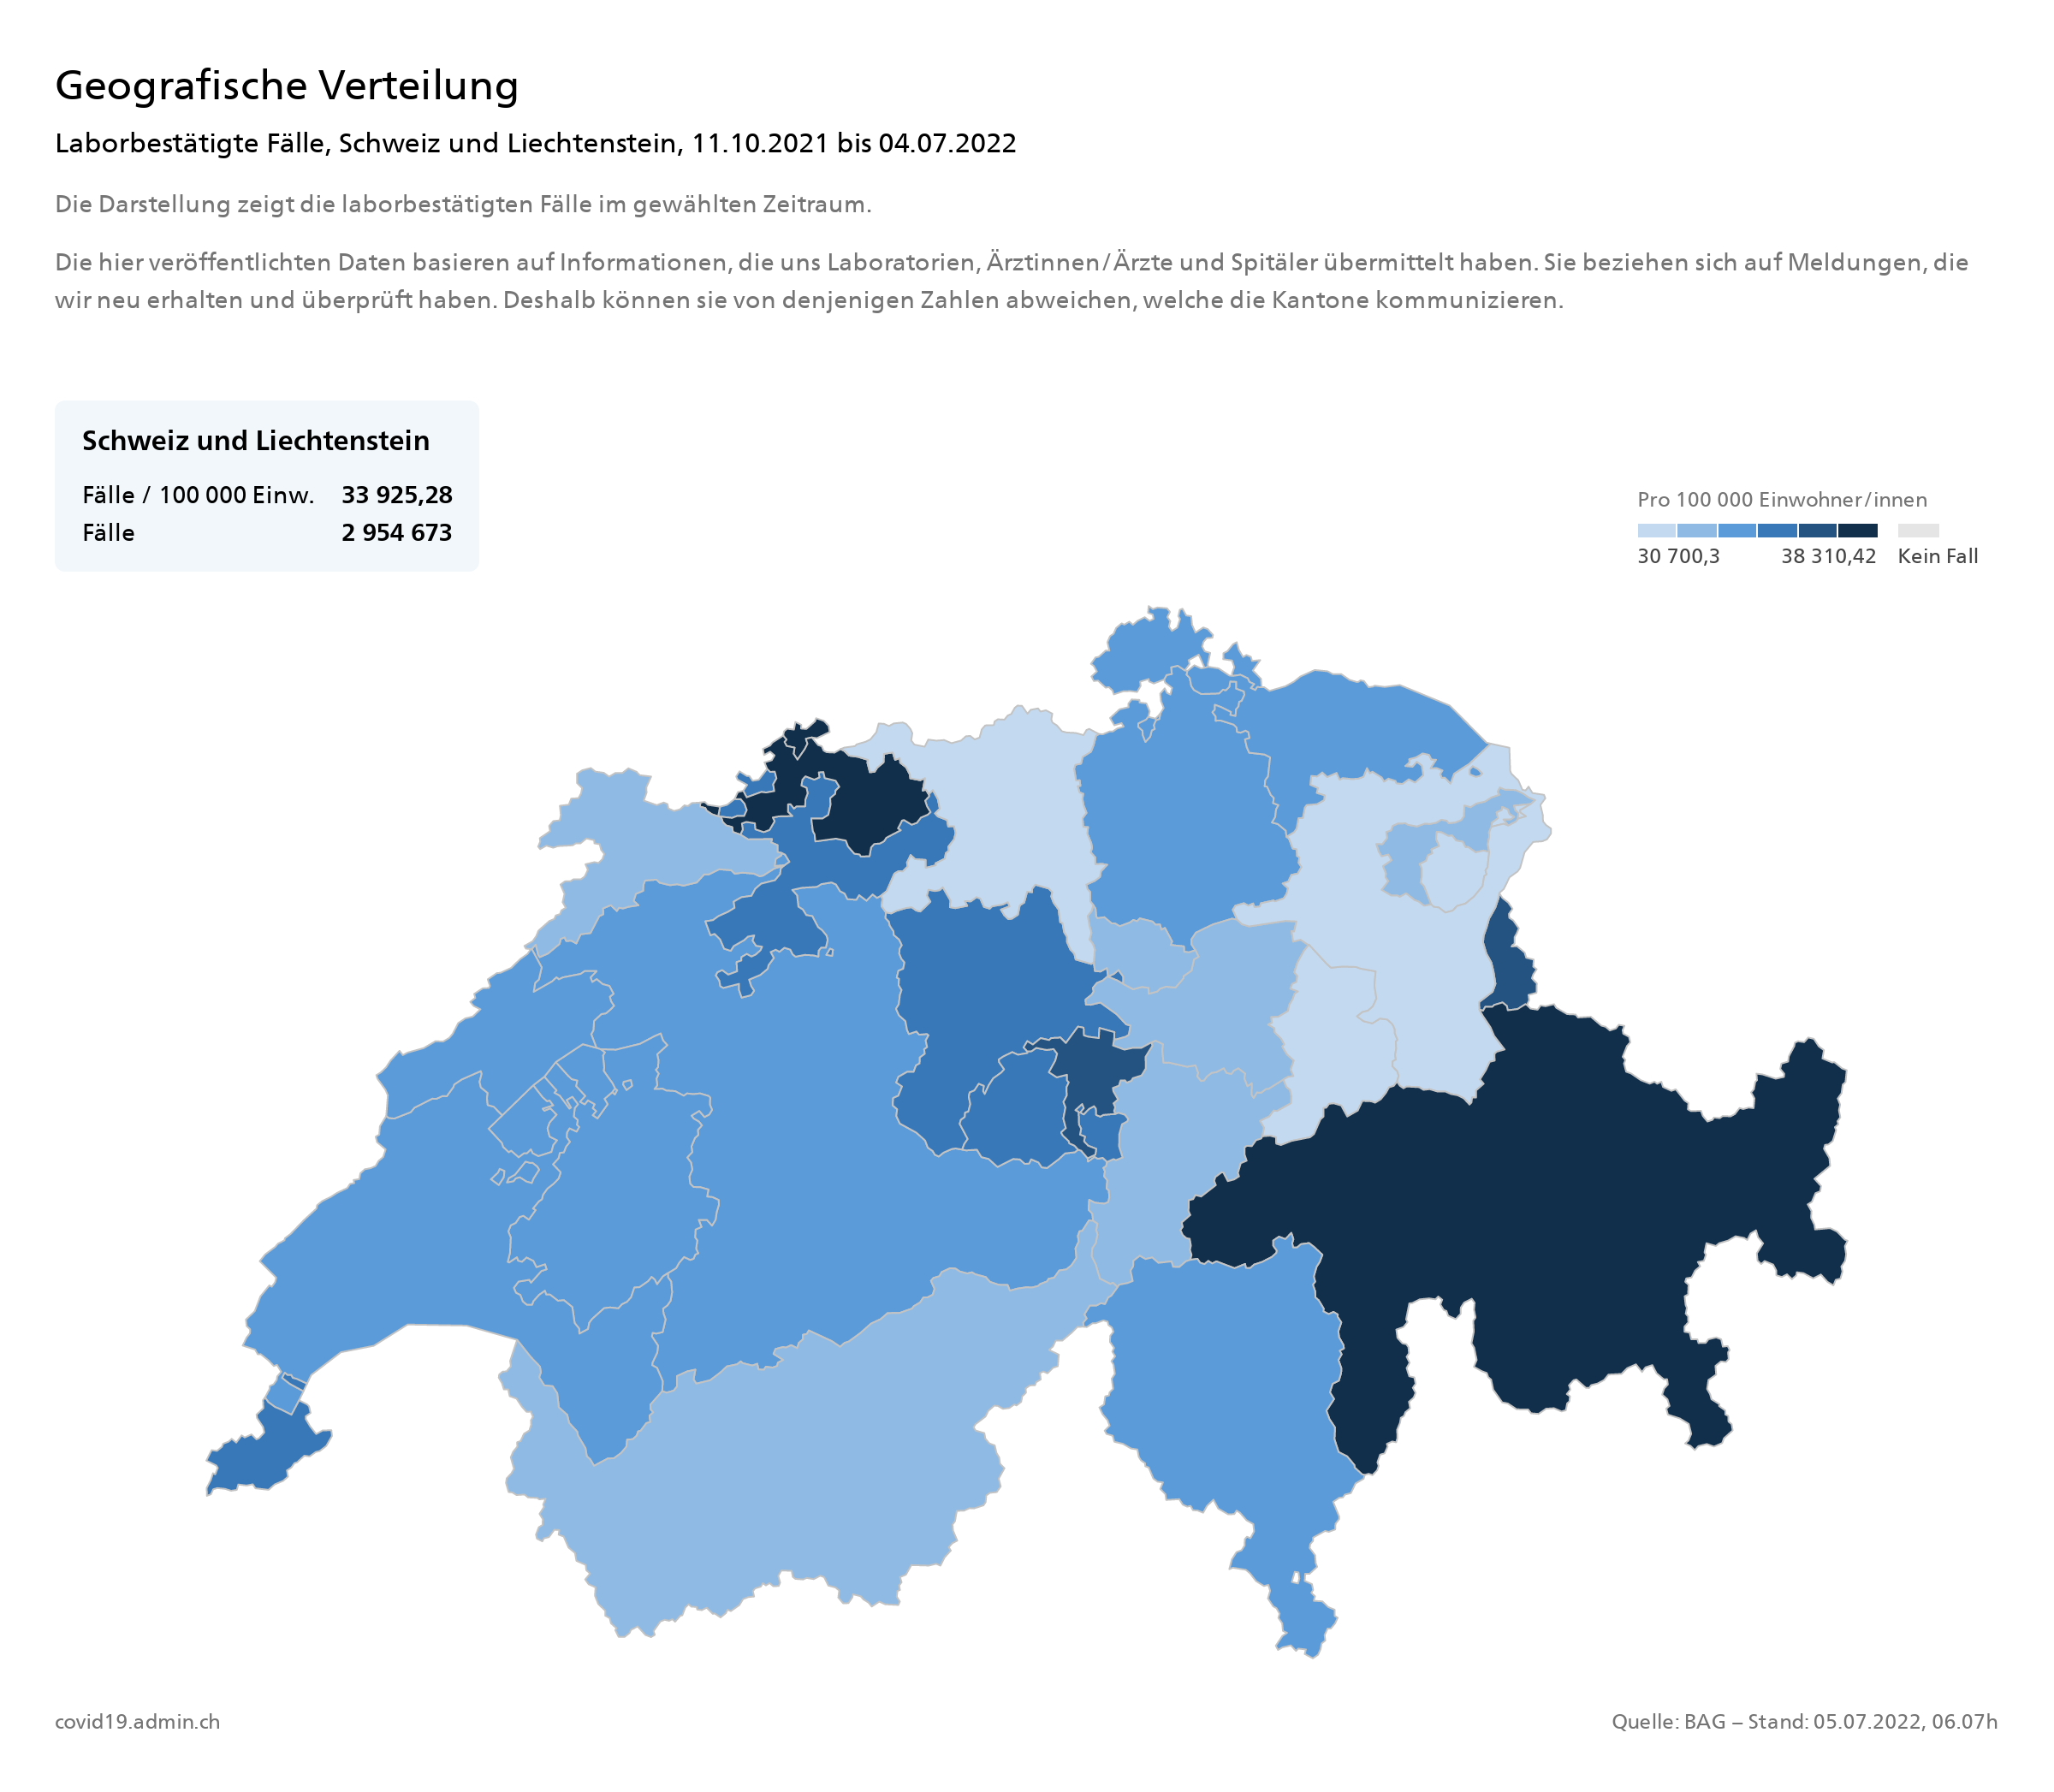
\includegraphics[width=12cm]{images/covid_dashboard_switzerland_choropleth_map.png}
    \centering
    \caption{Corona Virus Dashboard der Schweiz - Gebietsstufenkarte ~\citep{corona_dashboard_switzerland}}
    \label{fig:covid_dashboard_switzerland_choropleth_map}
\end{figure}

Als zusätzliche Visualisierungen wurden von den Probanden Radar Charts, sowie die Integration von Textelementen gewünscht.

\clearpage
\noindent
\textbf{Personalisierungsmöglichkeiten und Identifikation der Plattform}
\newline
\indent
80\% der befragten Personen bevorzugen die Möglichkeit, eigene Datenvisualisierungen hinzuzufügen und somit ihr persönliches Dashboard gestalten zu können. Diese Möglichkeit wäre gemäss den Probanden vor allem in der Corona Anfangszeit spannend gewesen. Rund 60\% der befragten Probanden gaben zudem an, dass Sie gerne Anpassungen am Design in Bezug auf Farben und Schriften vornehmen würden. Den restlichen Probanden sind Design Anpassungen nicht wichtig, als Begründung wurde hierbei genannt, dass das Design vom Anbieter selbst vorgegeben sein sollte.

Bei der Erstellung von Dashboards bevorzugen die Probanden die Verwendung von Vorlagen. Hierbei sollen die Vorlagen nach bestimmten Kategorien geordnet sein.

Als primäre Anwendungsplattform wurde von den Millenials die Umsetzung als eigenständige App sowie als Webseite mit Responsive Design (dynamische Anpassung des Layouts an Hand der Bildschirmgrösse) präferiert.\\

\noindent
\textbf{Sharingmöglichkeiten}
\newline
\indent
Die Sharingfunktionalität wurde von rund 80\% der Probanden als sinnvoll erachtet, jedoch eher im Rahmen einer Zusatzfunktionalität (``nice to have``).


\subsubsection{Definition der Anforderungen}
Aufgrund der evaluierten Ergebnisse des Online Fragebogens sowie den Rückmeldungen aus den durchgeführten Interviews werden vom Autor nachfolgend die relevanten Anforderungen spezifiziert.\\

\noindent
\textbf{Wahl der Plattform}
\newline
\indent
Die Umsetzung soll als Web Applikation erfolgen. Mithilfe von Responsive Design soll ebenfalls die Möglichkeit geschaffen werden, das Artefakt auf dem Smartphone zu nutzen.\\

\noindent
\textbf{Datenauswahl und Datenvisualisierungen}
\newline
\indent
Aufgrund der identifizierten Kategorien (siehe Tabelle \ref{table:interest_per_category}) wurde beschlossen, dass sich die Datenvisualisierungen auf den Bereich ``Ìnformationen zum Schweregrad der Pandemien`` fokussieren. Konkret stehen hierbei Spitalauslastung sowie Todesfälle in Bezug auf Corona im Fokus. Als Datenvisualisierungen werden Liniendiagramme, Balkenendiagramme sowie Gebietsstufenkarten berücksichtigt.\\

\clearpage
\noindent
\textbf{Filtermöglichkeiten}
\newline
\indent
In Bezug auf die Filtermöglichkeiten soll der Fokus auf Zeit- und Regionsbasierte Filterung gelegt werden. Der Nutzer soll jederzeit einen schnellen Zugriff auf den Filterbereich haben (``mitfliessen`` des Filters).\\

\noindent
\textbf{Personalisierungsmöglichkeiten}
\newline
\indent
Beim Erstellen des Dashboards soll der Nutzer die Möglichkeit besitzen sein Dashboard aufgrund einer Vorlage zu erstellen. Die Vorlagen sollen hierbei einem thematischen Bereich zugeordnet sein. Beim Gestalten des Dashboards soll der Nutzer die Möglichkeit besitzen, dynamisch neue Visualisierungen hinzuzufügen.\\

\noindent
\textbf{Aufbau der Bereiche}
\newline
\indent
Das Artefakt soll hierbei über folgende relevante Bereiche verfügen:
\begin{itemize}
    \item Willkommensseite welche den Sinn und Zweck der Anwendung aufzeigt
    \item Bereich in welchem Dashboards verwaltet werden können
    \item Bereich in welchem Dashboards gestaltet werden können
    \item \gls{faq} Bereich mit Informationen zu Corona
\end{itemize}


\clearpage
\section{Design und Development}
TODO

\subsection{Design mittels Sketching}
TODO

\subsection{High-Fidelity Prototyp als Web Applikation}
TODO

\clearpage
\section{Auswertung}
TODO

\clearpage
\section{Fazit}
TODO

\clearpage
\section{Reflexion und Limitationen}
TODO

\clearpage
\bibliographystyle{apacite}
\urlstyle{rm}
\bibliography{ref}

\clearpage
\appendix
\section{Rechercheprotokoll}
\begin{table}[ht]
	\begin{tabular}{@{}p{4cm}p{4cm}p{6.5cm}@{}}
		\toprule
		\textbf{Quelle} & \textbf{Schlüsselwörter}        & \textbf{Artikel}        \\ \midrule
		\url{https:                                                                 \\scholar.google.com}                         & covid dashboard                 & ~\citep{dong}         \\ \midrule
		                &                                 & ~\citep{florez}    \\ \midrule
		                &                                 & ~\citep{berry}     \\ \midrule
		                & user centered dashboards        & ~\citep{francois}  \\ \midrule
		                &                                 & ~\citep{young}     \\ \midrule
		                & customizable dasbhoards         & ~\citep{roberts}   \\ \midrule
		\url{https:                                                                 \\dl-acm.org}                                 & covid19 dashboard               & ~\citep{vitale}           \\ \midrule
		                & evaluating crisis dashboards    & ~\citep{ivanov}    \\ \midrule
		                & data dashboards                 & ~\citep{maheshwari.}    \\ \midrule
		                &                                 & ~\citep{beheshti}      \\ \midrule
		\url{https:                                                                 \\google.com}                                 & covid dashboard evaluation      & ~\citep{barbazza}         \\ \midrule
		                & how user use covid19 dashboards & ~\citep{ivankovic} \\ \bottomrule
	\end{tabular}
	\caption{\label{tab:research-protocol}Rechercheprotokoll (Eigene Darstellung)}
\end{table}

\clearpage
\section{Zeitplan}

\begin{table}[ht]
	\begin{tabular}{@{}p{13cm}p{2cm}@{}}
		\toprule
		\textbf{Tätigkeit}                                                                                & \textbf{Stichtag} \\ \midrule
		Erstellung des Untersuchungsinstrumentes                                                          & 08.05.2022        \\ \midrule
		Kapitel Einleitung fertig stellen                                                                 & 08.05.2022        \\ \midrule
		Kapitel Problemidentifizierung und Motivation fertig stellen                                      & 15.05.2022        \\ \midrule
		Durchführung der teilstrukturierten Interviews mit Hilfe des erstellten Untersuchungsinstrumentes & 29.05.2022        \\ \midrule
		Abgabe Exposé                                                                                     & 22.05.2022        \\ \midrule
		Kapitel Identifikation der Ziele fertig stellen                                                   & 05.06.2022        \\ \midrule
		Implementierung Prototyp                                                                          & 26.06.2022        \\ \midrule
		Kapitel Design und Development fertig stellen                                                     & 26.06.2022        \\ \midrule
		Kapitel Fazit fertig stellen                                                                      & 03.07.2022        \\ \midrule
		Kapitel Reflexion und Limitation fertig stellen                                                   & 10.07.2022        \\ \midrule
		Korrekturlesung und Verbesserung                                                                  & 24.07.2022        \\ \midrule
		Abgabe Thesis                                                                                     & 25.07.2022        \\ \bottomrule
	\end{tabular}
	\caption{\label{tab:time-table}Zeitplan (Eigene Darstellung)}
\end{table}

\clearpage
\section{Leitfaden für teilstrukturierte User Interviews}

\subsection{Einleitung}
Als Teil meiner Bachelorarbeit untersuche ich die Konzeption sowie Erstellung eines personalisierbaren Corona-Dashboards für Millennials. Dieses Interview hilft mir dabei drei relevante Fragestellungen in diesem Zusammenhang zu klären. Hierbei ist es wichtig zu erwähnen, dass Sie sich keine Sorgen um korrekte oder inkorrekte Aussagen machen müssen, die besten Antworten sind ihre persönlichen Meinung. Als Erstes sehen wir uns an, welche Informationen in Bezug auf Corona Sie für relevant halten und welche Datenvisualisierungen Sie bevorzugen. Zum Schluss halten wir noch die für Sie wichtigsten Personalisierungsmöglichkeiten fest. Bevor wir jedoch beginnen möchte ich Ihnen noch kurz den Fachbegriff Dashboard erläutern
\\

\textit{Fachbegriff Dashboard}
\\
Der Begriff Dashboard kommt aus der Automobilindustrie und bezeichnet die Frontkonsole (das Dashboard) Ihres Fahrzeugs. Auf dieser sind die wichtigsten Informationen wie Geschwindigkeit, Ölstand etc. auf einen Blick ersichtlich. Dashboards sind also eine Zusammenstellung von verschiedenen Visualisierungen, welche die für Sie relevanten Informationen auf einen Blick ersichtlich machen.\\


\textit{Administrativer Teil}
\\
Kommen wir nun noch kurz zum administrativen Teil. Wie Sie bereits im Vorfeld informiert worden sind, wird dieses Meeting aufgezeichnet. Dies beinhaltet dabei sowohl Ton als auch das Video auf Ihrem Computer. Diese Aufnahmen werden jedoch nicht veröffentlicht, sondern dienen lediglich als Grundlage für Auswertungszwecke im Rahmen dieser Arbeit.\\\\
\textbf{WICHTIG: AUFNAHME STARTEN}


\clearpage
\subsection{Hauptteil}

\textit{Hauptfragen}
\begin{itemize}
    \item Untergeordnete Forschungsfrage 1 und 2 wird via Online Formular beantwortet: \url{https://forms.gle/JdErDGAQ2YkwPZe57}
    \item Untergeordnete Forschungsfrage 3 wird mittels think-aloud Ansatz beantwortet, hierbei wird der Nutzer aufgefordert folgendes Dashboard zu besuchen \url{https://www.covid19.admin.ch/de/overview}
    \begin{itemize}
        \item Was hat Ihnen an diesem Dashboard gefallen?
        \item Was hat Ihnen an diesem Dashboard nicht gefallen?
        \item Was würden Sie sich von diesem Dashboard persönlich wünschen?
        \item Welche Visualisierungen haben Ihnen besonders gefallen und warum?
        \item Gibt es noch andere Visualisierungen welche Sie noch ergänzen möchten (Twitter Feed, Corona Richtlinien in der unmittelbahren Umgebung via GPS)?
        \item Würden Sie es bevorzugen, wenn Sie selbst ein eigenes Dashboard kreieren könnten, sprich eigene Visualisierungen hinzuzufügen?
        \item Ist es Ihnen wichtig, dass Design an Ihre eigenen Bedürfnisse anpassen zu können?
        \item (Nur wenn Anpassung Design wichtig) Welche Aspekte des Designs wollen Sie anpassen können (Farbgebung, Schrift, Titel der Visualisierungen)?
        \item Würden Sie ein leeres Dashboard bevorzugen, auf welchem Sie Ihre eigenen Visualisierungen platzieren können?
        \item Wünschen Sie sich Vorlagen, bzw. Vorschläge von bereits fertig gestellten Dashboards für bestimmte Zwecke (zum Beispiel Über den Schweregrad der Pandemie informieren)?
        \item Sind Ihnen Filterfunktionalitäten wichtig, wenn ja welche (Region, Zeit etc.)?
        \item Würden Sie gerne die Visualisierungen mit Freunden teilen können?
        \item Würden Sie eher eine Desktop Applikation, eine Website oder eine App bevorzugen und warum?
        \item Hätten Sie persönlich Interesste, an der Evaluation eines solchen Prototypen teilzunehmen?
    \end{itemize}
\end{itemize}


\subsection{Schlussteil}
\begin{itemize}
    \item Wünschen Sie noch etwas zu ergänzen oder etwas mitzuteilen?
\end{itemize}

\textbf{WICHTIG: EINWILLIGUNGSERKLÄRUNG PER E-MAIL SENDEN}

\clearpage
\section{Leitfaden für Remote Lab Usability Testing}

\subsection{Einleitung}
Im Rahmen meiner Bachelor Arbeit habe ich eine Web Applikation entwickelt, welchen es Nutzern erlaubt ihr persönliches Corona Dashboard zu erstellen. Ihm Rahmen dieses Usability Testing würde mich interessieren, wie Sie eine solche Applikation nutzen würden.
\\

\textit{Administrativer Teil}
\\
Kommen wir nun noch kurz zum administrativen Teil. Wie Sie bereits im Vorfeld informiert worden sind, wird dieses Meeting aufgezeichnet. Dies beinhaltet dabei sowohl Ton als auch das Video auf Ihrem Computer. Diese Aufnahmen werden jedoch nicht veröffentlicht, sondern dienen lediglich als Grundlage für Auswertungszwecke im Rahmen dieser Arbeit\\\\
\textbf{WICHTIG: AUFNAHME STARTEN}


\clearpage
\subsection{Hauptteil}

\textit{Warm-Up Fragen}
\begin{itemize}
    \item Haben Sie bereits persönliche Erfahrungen mit Applikationen die ihnen erlauben ihr eigenes Dashboard zu erstellen?
\end{itemize}

\textit{Task 1: Willkommensseite}
\begin{itemize}
    \item Wie finden Sie prinzipiell die hier aufgeführten Hauptbereiche entsprechen diese Ihren Vorstellungen, vermissen Sie gewisse Punkte?
    \item Wo würden Sie klicken um ihr eigenes Dashboard erstellen zu können?
\end{itemize}

\textit{Task 2: Dashboard erstellen}
\begin{itemize}
    \item Klicken auf \textbf{Create a Dashboard}
    \item Name eingeben
    \item Vorlage (beobachten was Nutzer instinktiv tut)
    \item Schauen ob Nutzer auf Create a Dashboard oder auf Create and Edit klickt
\end{itemize}

\textit{Task 3: Dashboard gestalten}
\begin{itemize}
    \item Klick auf Plus Button
    \item Widget aus dem Dialog auswählen
    \begin{itemize}
        \item Covid Deaths Over Time - Line Chart
        \item Sum of Covid Deaths over Time - Line Chart
        \item Sum of Covid Deaths Total - Bar Chart
        \item Hospital Capacity - Map
        \item Hospital Capacity - Bar Chart
    \end{itemize}
    \item Versuchen Widget zu verschieben (schauen ob Bleistift Symbol verstanden wird)
    \item Versuchen Widget zu vergrössern
    \item Versuchen Widget zu löschen
    \item Versuchen Edit Mode zu deaktivieren und fragen was Nutzer bei deaktiviertem Edit Mode erwarten
    \item Schauen ob Nutzer selbst darauf kommen dass Sie bei Liniendiagrammen zoom können
\end{itemize}

\textit{Task 4: Filtern}
\begin{itemize}
\item Versuchen zu filtern (schauen wo Nutzer klickt)
    \begin{itemize}
        \item Regionen auswählen welche von Interesse sind (Vorschlag SZ, TG, TI, ZH)
        \item Zeitbereich auswählen welcher von Interesse ist (Vorschlag: 01.03.2020 - 31.05.2020)
        \item Schauen wie der Nutzer auf Fehlerhinweise (keine Region ausgewählt etc. reagiert, mehr als 4 Regionen)
        \item Schauen ob Nutzer verstehen, dass Sie auf Save Time Range klicken müssen und ihn erst dann auswählen können
        \item Schauen ob Nutzer verstehen, dass Sie auf Apply Filter klicken müssen
        \item Schauen wie Nutzer einen Zeitfilter wechseln würden
        \item Schauen wie Nutzer einen Zeitfilter löschen würden
        \item Zeitbereich einstellen bei dem es keine Daten gibt und schauen was Nutzer erwarten würden
    \end{itemize}
\end{itemize}

\textit{Task 5: Speichern}
\begin{itemize}
\item Wo würden Nutzer klicken um zu speichern
\item Was erwarten Nutzer, dass gespeichert werden soll (Zoom Bereich bei Trends), Filter etc.
\end{itemize}

\textit{Task 6: Dashboard Overview}
\begin{itemize}
\item Was halten Sie von der Dashboard Übersicht?
\item Wo würden Sie klicken um Ihr Dashboard zu teilen (auffordern zu klicken)
\item Wo würden Sie klicken um Ihr Dashboard zu löschen (auffordern zu klicken)
\item Neuen Browser Tab öffnen und den Share-Link aus dem Clipboard einfügen
\item Notieren wie Nutzer nun reagiert (er hat das geteilte Dashboard gerade gelöscht)
\end{itemize}

\textit{Task 7: FAQ}
\begin{itemize}
\item Wie finden Sie den Aufbau / Layout?
\item Vermissen Sie etwas (Suchfunktion etc.)?
\end{itemize}

\textit{Task 8: About}
\begin{itemize}
\item Wie finden Sie den Aufbau / Layout?
\item Vermissen Sie etwas?
\end{itemize}


\subsection{Schlussteil}
\begin{itemize}
    \item Sind Ihnen die Notifications im unteren Bereich aufgefallen
    \item Wie haben Sie die Filterfunktionalität gefunden, hat Sie etwas daran gestört (z.Bsp. Filter Parameter sollten Global sichtbar sein ohne Sidenav aufklappen zu müssen etc.)
    \item Hätten Sie eine Filterinformation pro Widget gewünscht (als Overlay Toggle etc.)
    \item Wünschen Sie noch etwas zu ergänzen oder etwas mitzuteilen?
\end{itemize}

\textbf{WICHTIG: EINWILLIGUNGSERKLÄRUNG PER E-MAIL SENDEN}

\clearpage
\section{Eigenständigkeitserklärung}
Hiermit bestätigt der Verfasser, dass die vorliegende Arbeit selbstständig verfasst und keine anderen als die angegebenen Hilfsmittel benutzt wurden. Stellen der Arbeit, die dem Wortlaut oder dem Sinn nach anderen Werken entnommen sind, wurden unter Angaben der Quelle kenntlich gemacht.

\begin{figure}[ht]
	
\includegraphics[width=6cm]{images/signature.png}
\end{figure}
Yannick Hutter, Mels am 01. Mai 2022

\end{document}